\documentclass[../../main.tex]{subfiles}

\begin{document}
\chapter{正则系综的若干应用}

\section{态密度——配分函数的另一种形式}


无论是系统的配分函数亦或单粒子配分函数，它们的计算都是对态求和。从实操的角度来说，求和是一个不怎么友好的运算，它的近邻积分是一种更好的数学运算方式，因此我们这里提出另一种形式的配分函数，它是由积分表示的。

前文提到过一种计算配分函数的思路，我们把对态求和分成两步，第一步固定系统的能量，进行对态求和，第二步对系统所有可能的能量求和。第一步中我们要找到系统能量取某个值时的微观状态数，这其实就是系统某个能级的简并度，因此按照这种思路配分函数可以写成
\begin{equation}\label{eq:求和配分函数}
    Z=\sum_i g_i\mathrm{e}^{-\beta E_i}
\end{equation}
其中\(E_i\)表示系统的第\(i\)个能级，\(g_i\)表示这一能级的简并度。因此这种形式的配分函数相当于把对态求和合并同类项，变成对能级求和。

读者不难看出，这种形式的配分函数是没有实操性的，因为我们要计算系统能量为定值时的微观状态数，这正是微正则系综面临的数学难题。回想前文我们用微正则系综框架处理经典理想气体，我们先计算了一定能量范围内的量子态个数，但这个能量范围是人为引入的，所幸借助高维几何空间的特殊性质我们巧妙地避开了对能量宽度的定量讨论。微正则系综认为系统能量固定，因此引入能量范围是额外的人为操作，但是正则系综视角下，系统的能量是不固定的，计算一定能量范围内的量子态个数是完全合理的。进一步我们认为这个能量范围内的量子态它们的能量相同，那么配分函数可写成\footnote{表达式中的积分下限要根据具体的模型调整，这里做理论分析统一认为能级下限为\(0\)}
\begin{equation}\label{eq:积分配分函数}
    Z=\int_0^{\infty}g(E)\mathrm{e}^{-\beta E}\dd E
\end{equation}
其中\(g(E)\dd E\)表示系统能量在\(E\sim E+\dd E\)这个范围内的量子态个数。我们称\(g(E)\)为态密度，注意这不是简并度，可以理解为单位能量内的简并度。

关于态密度的计算，我们将在具体的模型中具体分析。值得讨论的是，把配分函数写成积分形式的条件是什么？不难发现，我们假定了\(\dd E\)这个能量范围内的量子态能量相同，也就是说近似认为相邻两个能级的能量相等，但这貌似有点牵强\footnote{假如真的这样假设，不断递推就会得到所有能级近似相等}，而且是不必要的。配分函数即式\eqref{eq:求和配分函数}是对\(\mathrm{e}^{-\beta E_i}\)求和而不是对能级本身求和，因此我们只需假定相邻两个能级的\(\mathrm{e}^{-\beta E_i}\)近似相等，也就是说它们的相对误差远远小于1
\begin{equation}
    \abs{\frac{\mathrm{e}^{-\beta E_{i+1}}-\mathrm{e}^{-\beta E_i}}{\mathrm{e}^{-\beta E_i}}}=\abs{\mathrm{e}^{-\beta (E_{i+1}-E_i)}-1}\ll 1
\end{equation}
巧妙的是，倘若\(\beta (E_{i+1}-E_i)\ll 1\),那么
\begin{equation}
    \abs{\mathrm{e}^{-\beta (E_{i+1}-E_i)}-1}\approx \abs{-\beta (E_{i+1}-E_i)}\ll 1
\end{equation}
这正是我们需要的近似条件，也就是说\(\beta (E_{i+1}-E_i)\ll 1\)就是我们把配分函数从求和变成积分的条件。不妨假设系统能级间隔的量级为\(\Delta E\)，那么这个条件可以写作
\begin{equation}
    \Delta E\ll kT
\end{equation}
这个条件被不少教材称为能量准连续条件。但笔者认为这个称呼并不恰当，因为我们的积分式\eqref{eq:积分配分函数}中的\(g(E)\dd E\)表示的就是量子态的个数，这正是能量量子化的结果。此外从单纯的计算角度来说，配分函数的求和其实是积分的左矩形近似，要让两者近似相等，需要\(\beta\)尽可能的小即温度尽可能的高，所以不妨直接称呼这个近似条件为高温条件。正因为积分形式的配分函数\eqref{eq:积分配分函数}是有条件的，在数学允许的情况下我们应使用求和式\eqref{eq:求和配分函数}，在使用积分形式的时候一定要判断是否满足高温条件。提醒读者注意，态密度这一概念不依赖宏观系统而存在，态密度也不会随系统的温度而改变，它是纯力学的物理量。温度影响的是用态密度积分来计算配分函数的准确性，温度太低时，用它计算配分函数偏差较大，但态密度本身仍有意义。

到这里我们所有的讨论都是针对系统的配分函数，不难想到，同样的近似方法也可以应用到单粒子配分函数上，只是讨论对象从系统的能级变成单粒子能级，同样我们可以定义一个单粒子态密度。在统计物理课程中，单粒子态密度是更常使用的。下面我们通过一个例子体会一下两种配分函数计算的差别。
\begin{example}
    计算谐振子的单粒子配分函数。分别使用求和形式和积分形式，给出积分形式趋近求和形式的条件。
    \begin{solution}
        谐振子的能级为\(E_n=\left(n+\frac{1}{2}\right)\hbar\omega\)且每个能级都是非简并的，因此单粒子配分函数是
        \begin{equation}
            Z_1=\sum_{n=0}^{\infty} \mathrm{e}^{-\beta\left(n+\frac{1}{2}\right)\hbar\omega}=\mathrm{e}^{-\frac{1}{2}\beta\hbar\omega}\sum_{n=0}^{\infty}\left(\mathrm{e}^{-\beta\hbar\omega}\right)^n=\mathrm{e}^{-\frac{1}{2}\beta\hbar\omega}\frac{1}{1-\mathrm{e}^{-\beta\hbar\omega}}
        \end{equation}
        上式中的无穷求和本质是等比数列求和，更高级的表示即几何级数\(\displaystyle\frac{1}{1-z}=\sum_{n=0}^{\infty}z^n\;\abs{z}<1\)，因为\(\beta>0\)所以上式的求和显然满足收敛条件。

        接下来我们用积分方法来计算单粒子配分函数，我们先计算出结果再讨论积分方法成立的条件。我们不直接使用式\eqref{eq:积分配分函数}，考虑到谐振子能级取决于\(n\)，那么一定能量范围内的量子态个数，可以引伸出一个“一定\(n\)范围内的量子态个数”这一概念，进而我们给出下述形式的谐振子单粒子配分函数
        \begin{equation}\label{eq:谐振子积分配分函数}
            Z_1=\int_0^{\infty}g(n)\mathrm{e}^{-\beta\left(n+\frac{1}{2}\right)\hbar\omega}\dd n
        \end{equation}
        其中\(g(n)\)表示\(n\)在\(n\sim n+\dd n\)这个范围内时粒子的量子态个数。注意这里的\(g(n)\)和式\eqref{eq:积分配分函数}中的\(g(E)\)是两个函数，只是两个函数用了同一个符号表示\footnote{这就是符号混乱，但不少教科书中都采用这种写法}，因为它们物理本质是相同的，均表示量子态的密度。为了细致的研究一下这两个函数的关系，我们记\(g(n)\)为\(h(n)\)。上式实际上只是式\eqref{eq:积分配分函数}换元后的形式，不妨记\(E=f(n)\)
        \begin{equation}
            \begin{split}
                Z_1&=\int_0^{\infty}g(E)\mathrm{e}^{-\beta E}\dd E \\
                &\xlongequal{E=f(n)}\int_0^{\infty}g(f(n))\mathrm{e}^{-\beta f(n)}f'(n)\dd n \\
                &=\int_0^{\infty}g(f(n))f'(n)\mathrm{e}^{-\beta f(n)}\dd n \\
                &=\int_0^{\infty}h(n)\mathrm{e}^{-\beta f(n)}\dd n
            \end{split}
        \end{equation}
        不难看出式\eqref{eq:谐振子积分配分函数}中的\(g(n)\)即上式中的\(h(n)\)确实和\(g(E)\)是不一样的。可以看出两者的转化关系是
        \begin{equation}
            g(n)\dd n=g(E)\dd E=g(f(n))f'(n)\dd n
        \end{equation}
        这并不难理解，因为\(g(n)\dd n\)和\(g(E)\dd E\)均表示一定范围内的量子态个数，只是前者用\(n\)标记范围，后者用\(E\)标记范围。实际上在计算具体模型的配分函数时往往不会使用式\eqref{eq:积分配分函数}这个原始形式，我们往往会找一个新变量表示能量，再计算出关于这个变量的量子态密度。

        让我们回到谐振子的话题上。\(g(n)\dd n\)表示\(n\)在\(n\sim n+\dd n\)这个范围内时谐振子的量子态个数，对于量子态分布如此明确的谐振子，这句话有点略显奇怪，不过无所谓，我们借鉴微正则系综中处理经典理想气体的手法，采用平均的视角来计算。想象一个半实轴，每个自然数的位置就是一个量子态，显然平均而言一个量子态占据的大小是1，那么\(n\sim n+\dd n\)范围内的量子态个数就是这个范围本身的大小即\(\dd n\)，也就是\(g(n)\dd n=\dd n\)，计算出了态密度，就可以计算单粒子配分函数了
        \begin{equation}
            Z_1=\int_0^{\infty}\mathrm{e}^{-\beta\left(n+\frac{1}{2}\right)\hbar\omega}\dd n=\mathrm{e}^{-\frac{1}{2}\beta\hbar\omega}\int_0^{\infty}\mathrm{e}^{-\beta\hbar\omega n}\dd n
        \end{equation}
        上式的积分是很容易计算的，为了与求和形式的单粒子配分函数比较，我们把这个积分拆成无穷的积分的和
        \begin{equation}
            \begin{split}
                \int_0^{\infty}\mathrm{e}^{-\beta\hbar\omega x}\dd x&=\sum_{n=0}^{\infty}\int_n^{n+1}\mathrm{e}^{-\beta\hbar\omega x}\dd x\\
                &=\frac{1}{-\beta\hbar\omega}\sum_{n=0}^{\infty}\big[\mathrm{e}^{-\beta\hbar\omega (n+1)}-\mathrm{e}^{-\beta\hbar\omega n}\big] \\
                &=\frac{\mathrm{e}^{-\beta\hbar\omega}-1}{-\beta\hbar\omega}\sum_{n=0}^{\infty}\mathrm{e}^{-\beta\hbar\omega n}
            \end{split}
        \end{equation}
        那么显然有
        \begin{equation}
            Z_1(\text{积分})=\frac{\mathrm{e}^{-\beta\hbar\omega}-1}{-\beta\hbar\omega}\mathrm{e}^{-\frac{1}{2}\beta\hbar\omega}\sum_{n=0}^{\infty}\mathrm{e}^{-\beta\hbar\omega n}=\frac{\mathrm{e}^{-\beta\hbar\omega}-1}{-\beta\hbar\omega}Z_1(\text{求和})
        \end{equation}
        求和形式的配分函数是准确的，积分形式作为近似两者自然是不等的。不难发现，倘若\(\beta\hbar\omega\ll 1\)那么\(\mathrm{e}^{-\beta\hbar\omega}-1\approx-\beta\hbar\omega\)，此时积分结果趋近求和结果。对于谐振子来说，\(\Delta E\)正是\(\hbar\omega\)，所以积分形式的配分函数成立的条件如预期的是\(\Delta E\ll kT\)。值得注意的是，因为普朗克常数格外的小，所谓的“高温”是否是常识中的高温\footnote{正如高温超导实际上是低温超导}依赖于\(\omega\)的值。倘若取\(\omega=10^9 \text{Hz}\)，那么\(T\gg10^{-2}\text{K}\)，几十开尔文的温度就可以认为是高温了。倘若取\(\omega=10^{14} \text{Hz}\)，那么\(T\gg10^{3}\text{K}\)，确实是高温了。不过讨论谐振子的这一条件没什么实用价值，作为少数可以解析计算的配分函数，我们自然要使用解析求和解而不是积分近似解。
    \end{solution}
\end{example}

\section{经典理想气体}

\subsection{计算单粒子配分函数}
本节开始我们讨论如何用正则系综的手段处理经典理想气体。我们先讨论最简单的情形，即假设理想气体分子是单原子分子，只考虑它的平动。经典理想气体是满足非简并条件的，因此它的配分函数是\(Z=\frac{1}{N!}Z_1^{N}\)。利用求和计算单粒子配分函数是不行的，读者可以自行尝试，最后得到的求和式没有初等解，要依赖积分近似计算，因此我们一开始就使用态密度来计算单粒子配分函数。

单个理想气体分子的能级公式为\(E_{n_x,n_y,n_z}=\frac{\hbar^2\pi^2(n_x^2+n_y^2+n_z^2)}{2mL^2}\)，粗略地认为能级间隔为\(\Delta E\approx \frac{\hbar^2\pi^2}{2mL^2}\)，那么高温条件是
\begin{equation}
    T\gg \frac{\hbar^2\pi^2}{2mL^2k}
\end{equation}
取最轻的原子氢原子，\(m\approx10^{-27}\text{Kg}\)，取\(L=0.1\text{m}\)，那么\(T\gg 10^{-15}\text{K}\)，这个估计是粗略的，不过在极低的温度下，经典理想气体模型不再适用，我们要用量子统计，细究这个下限是没有意义的。对于室温上下的理想气体，高温条件显然是成立的。

为了计算理想气体分子的态密度，我们要稍微修改气体分子的能级公式。回想自由粒子能级公式的推导过程，不难理解如下表达式
\begin{equation}
    \begin{cases}
        \displaystyle E_{\bm{k}}=\frac{\hbar^2k^2}{2m} \\
        \displaystyle k^2=k_x^2+k_y^2+k_z^2 \quad k_x=\frac{n_x\pi}{L},k_y=\frac{n_y\pi}{L},k_z=\frac{n_z\pi}{L}
    \end{cases}
\end{equation}
其中\(k\)是波矢\(\bm{k}\)的大小，为了避免符号混乱，我们用\(\k\)表示玻尔兹曼常数。上式表示的含义可以这样理解。以\(\{k_x,k_y,k_z\}\)为轴建立直角坐标系，在\(k_x=\frac{n_x\pi}{L},k_y=\frac{n_y\pi}{L},k_z=\frac{n_z\pi}{L}\)处画出一个格点，那么显然每个格点都表示一个量子态，这个量子态的能量由格点到原点的距离决定。
\begin{figure}[H]
    \centering
    \includegraphics[width=0.45\textwidth]{./理想气体量子态示意图.pdf}
    \caption{\(\{k_x,k_y,k_z\}\)空间（常称为\(\bm{k}\text{空间}\)或动量空间）示意图，这个空间的每一个格点都表示一个量子态}
\end{figure}

基于这样的理解，我们先计算\(g(k)\dd k\)，它表示\(k\)在\(k\sim k+\dd k\)内的量子态个数。我们依旧采用平均的视角计算这个态密度。每个格点占据的空间大小为\(\left(\frac{\pi}{L}\right)^3\)，不难得到\(\dd k\)这个范围的大小为\(\frac{1}{8}4\pi k^2\dd k\)，\(\frac{1}{8}\)的来源是量子数\(\{n_x,n_y,n_z\}\)都是正整数，因此我们只讨论所有坐标均为正值的卦限\footnote{我们这里做的计算和微正则系综中处理理想气体时计算一定能量范围内的系统量子态个数完全一样，这里还要简单很多，因为我们处理的是单粒子而不是整个系统}。确定这两点后，可得态密度为
\begin{equation}
    g(k)\dd k=\frac{\frac{1}{8}4\pi k^2\dd k}{\left(\frac{\pi}{L}\right)^3}=\frac{L^3k^2\dd k}{2\pi^2}=\frac{Vk^2}{2\pi^2}\dd k
\end{equation}
这样的态密度是关于波矢大小的。前文我们已经讲述过，态密度表示一定范围内的量子态个数，这个范围可以用不同的变量标记，不同的态密度之间通过自变量的函数关系进行变换。由\(k=\sqrt{\frac{2mE}{\hbar^2}}\)不难得到关于能量的态密度
\begin{equation}
    g(E)\dd E=g(k)\dd k=\frac{Vk^2}{2\pi^2}\dd k=\frac{V}{2\pi^2}\frac{2mE}{\hbar^2}\sqrt{\frac{m}{2\hbar^2E}}\dd E
\end{equation}
我们不再进一步化简，不难看出\(g(E)\propto\sqrt{E}\)，也就是说可以认为简并度随能级的变化大致\footnote{不要细究具体的变化规律，从图\ref{fig:box-degeneracy}中可以看到简并度随能级是忽上忽下的，只有一个整体趋势}是抛物线形状。这正是我们在图\ref{fig:box-degeneracy}中猜出来的结论，那里我们利用数值计算，从图中看出了抛物线的趋势。

鉴于\(g(E)\dd E\)的表达式比较复杂，我们使用\(g(k)\dd k\)计算单粒子配分函数，即
\begin{equation}
    Z_1=\int_0^{\infty}g(E)\mathrm{e}^{-\beta E}\dd E=\int_0^{\infty}g(k)\mathrm{e}^{-\beta\frac{\hbar^2k^2}{2m}}\dd k
\end{equation}
带入具体的表达式可得
\begin{equation}
    Z_1=\frac{V}{2\pi^2}\int_0^{\infty}k^2\mathrm{e}^{-\frac{\beta\hbar^2}{2m}k^2}\dd k=\frac{V}{2\pi^2}\frac{\sqrt{\pi}}{4}\left(\frac{2m}{\beta\hbar^2}\right)^{\frac{3}{2}}=\frac{V}{\hbar^3}\left(\frac{m\k T}{2\pi}\right)^{\frac{3}{2}}
\end{equation}
计算中涉及的积分将由下面的例题给出。
\begin{example}
    计算\(\int_0^{\infty}x^2\mathrm{e}^{-\alpha x^2}\dd x\)
    \begin{solution}
        将高斯积分\(\int_0^{\infty}\mathrm{e}^{-\alpha x^2}\dd x=\frac{1}{2}\sqrt{\frac{\pi}{\alpha}}\)的左右两边对\(\alpha\)求导，则有
        \begin{equation}
            -\int_0^{\infty}x^2\mathrm{e}^{-\alpha x^2}\dd x=-\frac{1}{4}\sqrt{\pi}\alpha^{-\frac{3}{2}}
        \end{equation}
        化简则得
        \begin{equation}
            \int_0^{\infty}x^2\mathrm{e}^{-\alpha x^2}\dd x=\frac{\sqrt{\pi}}{4}\alpha^{-\frac{3}{2}}
        \end{equation}
    \end{solution}
\end{example}

单粒子配分函数是无量纲的，那么\(\frac{1}{\hbar^3}\left(\frac{m\k T}{2\pi}\right)^{\frac{3}{2}}\)就具有粒子数密度的量纲，我们称其为量子密度\(n_{\text{Q}}\)，也就是说
\begin{equation}
    Z_1=Vn_{\text{Q}}\qquad n_{\text{Q}}=\frac{1}{\hbar^3}\left(\frac{m\k T}{2\pi}\right)^{\frac{3}{2}}
\end{equation}
既然\(n_{\text{Q}}\)具有粒子数密度的量纲，那么\(\lambda_{\text{th}}=n_{\text{Q}}^{-\frac{1}{3}}\)就是长度的量纲，我们称其为热波长，这样配分函数还可以写成
\begin{equation}
    Z_1=\frac{V}{\lambda_{\text{th}}^3}\qquad \lambda_{\text{th}}=\hbar\sqrt{\frac{2\pi}{m\k T}}
\end{equation}
在巨正则系综部分我们会看到，经典理想气体满足非简并极限的本质就是\(n\ll n_{\text{Q}}\)或者说\(n\lambda_{\text{th}}^3\ll 1\)。

有意思的是，当自由粒子满足非简并条件时，其一定满足高温条件。我们把非简并条件的两边取\(\frac{2}{3}\)次幂，可得
\begin{equation}
    T\gg\frac{2\pi\hbar^2N^{\frac{2}{3}}}{mL^2\k}
\end{equation}
将上式与高温条件的右式作比可得
\begin{equation}
    \frac{2\pi\hbar^2N^{\frac{2}{3}}}{mL^2\k}\frac{2mL^2\k}{\hbar^2\pi^2}=\frac{4N^{\frac{2}{3}}}{\pi}\gg 1\Longrightarrow \frac{2\pi\hbar^2N^{\frac{2}{3}}}{mL^2\k}\gg \frac{\hbar^2\pi^2}{2mL^2\k}
\end{equation}
可以看到，对于经典理想气体，它能被看成经典理想气体这一物理上的近似比计算单粒子配分函数时把求和变成积分这一数学近似手段更重要。实际上后文我们处理量子理想气体时，非简并条件已不再满足，但我们还会使用把求和变积分这一数学近似。

\subsection{经典理想气体的态函数}
经典理想气体系统的配分函数由\(Z=\frac{1}{N!}Z_1^{N}\)给出，即
\begin{equation}
    Z=\frac{1}{N!}\frac{V^N}{\hbar^{3N}}\left(\frac{m\k T}{2\pi}\right)^{\frac{3N}{2}}
\end{equation}
从配分函数出发求偏导就能得到各热力学量，这是纯粹的数学计算，希望读者自己尝试形成自己的风格。

我们先计算系统的内能
\begin{equation}
    \begin{split}
        U=-\pdv{\ln Z}{\beta}=-N\pdv{\ln Z_1}{\beta}&=-N\pdv{\beta}\left(\ln\frac{V}{\hbar^3}+\frac{3}{2}\ln\frac{m}{2\pi\beta}\right) \\
        &=-N\frac{3}{2}\frac{2\pi\beta}{m}\left(-\frac{m}{2\pi\beta^2}\right) \\
        &=\frac{3}{2}N\k T=\frac{3}{2}nRT
    \end{split}
\end{equation}
这一结果是毫无意外地，显然定容热容为\(C_V=\frac{3}{2}nR\)。接着我们计算系统的自由能
\begin{equation}
    \begin{split}
        F=-\k T\ln Z&=-N\k T\ln Z_1+N\k T\ln N-N\k T \\
        &=-N\k T\ln\frac{V}{\hbar^3}-\frac{3}{2}N\k T\ln\frac{m\k T}{2\pi}+N\k T\ln N-N\k T
    \end{split}
\end{equation}
求出特性函数后，其余热力学量通过特性函数的偏导计算
\begin{equation}
    p=-\left(\pdv{F}{V}\right)_{N,T}=\frac{N\k T}{V}=\frac{nRT}{V}
\end{equation}
这正是理想气体状态方程。接着计算理想气体的熵，因为\(\frac{1}{N!}\)的修正，我们预期得到的熵是广延量
\begin{equation}
    \begin{split}
        S=-\left(\pdv{F}{T}\right)_{N,V}&=N\k\ln\frac{V}{\hbar^3}+\frac{3}{2}N\k\ln\frac{m\k T}{2\pi}+\frac{3}{2}N\k-N\k\ln N+N\k \\
        &=N\k\ln\left[\frac{V}{N\hbar^3}\left(\frac{m\k T}{2\pi}\right)^{\frac{3}{2}}\right]+\frac{5}{2}N\k
    \end{split}
\end{equation}
显然这个熵和微正则系综中得到的熵完全相同，都是广延量。本小节计算的所有热力学量，和微正则系综给出的结果都是一致的，其中原因已在上一章分析过。从计算角度说，正则系综的处理难度是远小于微正则系综的，虽然两种系综都需要计算微观状态数，但在正则系综中我们只需计算一个单一粒子的微观状态数。而且我们得到的热力学量都是\((N,V,T)\)的函数，这样的热力学量很容易和实验对照。

最后我们计算一下理想气体的化学势，这是从未计算过的
\begin{equation}
    \begin{split}
        \mu=-\k T\pdv{\ln Z}{N}&=-\k T\pdv{N}(N\ln Z_1-N\ln N+N) \\
        &=-\k T(\ln Z_1-\ln N) \\
        &=-\k T\ln\frac{Z_1}{N}=-\k T\ln\left[\frac{V}{N\hbar^3}\left(\frac{m\k T}{2\pi}\right)^{\frac{3}{2}}\right]
    \end{split}
\end{equation}
上式中取对数的\(\frac{Z_1}{N}=\frac{Vn_{\text{Q}}}{N}=\frac{n_{\text{Q}}}{n}\gg 1\)，因此理想气体化学势为负，这也是可以预见的。根据热力学基本微分方程\(\dd U=T\dd S-p\dd V+\mu\dd N\)可得\(\mu=\left(\pdv{U}{N}\right)_{S,V}\)。我们假想两个系统\(A\)和\(B\)，两者的熵和体积完全相同而\(B\)系统比\(A\)系统多一个粒子。倘若两个系统能量相等，因为\(B\)系统多一个粒子，它的微观状态数会更多即熵更大，但我们要求两个系统的熵相同，因此\(B\)系统的能量一定要小于\(A\)系统，所以化学势必然是负的。
\subsection{双原子气体的热容}

本节我们要扩展我们的研究对象，研究更复杂的气体分子，双原子分子。原子物理课程学习过双原子分子的振转光谱，所以对于双原子分子，我们要考虑它的平动、振动和转动。我们的统计依旧从单粒子配分函数开始。为了让我们能够继续讨论这个话题，我们要假设双原子分子的这三种运动是相互独立的，也就是说双原子分子的平动不会改变它的转动、转动不会改变它的振动等等。仿照上一章组合配分函数的思路\footnote{从这些推导中读者应该能感受到，对于系统的不同成分，配分函数是这些成分的乘积，而热力学量的广延性要求结果是各成分的和，因此对配分函数取对数才可以得到热力学量是不意外的}，我们可以把单粒子配分函数拆成三个子配分函数。

假设双原子分子位于\(s\)量子态时，表征其平动、振动、转动的量子数分别为\(n_{\text{平}},n_{\text{振}},n_{\text{转}}\)，那么分子的能量就是\(E_s=E_{n_{\text{平}}}+E_{n_{\text{振}}}+E_{n_{\text{转}}}\)。三种运动的独立性意味着三种量子数毫无关系，那么
\begin{equation}
    Z_1=\sum_s \mathrm{e}^{-\beta E_s}=\sum_{n_{\text{平}},n_{\text{振}},n_{\text{转}}}\mathrm{e}^{-\beta E_{n_{\text{平}}}}\mathrm{e}^{-\beta E_{n_{\text{振}}}}\mathrm{e}^{-\beta E_{n_{\text{转}}}}=Z_{\text{平动}}Z_{\text{振动}}Z_{\text{转动}}
\end{equation}
不急于计算三种配分函数，我们先求热力学量的表达式，本节主要关注定容热容，不难想到热容应是这三部分的贡献之和。我们考虑的仍是经典理想气体，因此配分函数依旧是\(Z=\frac{1}{N!}Z_1^N\)，这给出内能公式
\begin{equation}
    U=-\pdv{\ln Z}{\beta}=-N\pdv{\ln Z_1}{\beta}=-N\pdv{\ln Z_{\text{平动}}}{\beta}-N\pdv{\ln Z_{\text{振动}}}{\beta}-N\pdv{\ln Z_{\text{转动}}}{\beta}
\end{equation}
显然，热容就是上述三项对温度的导数，即\(C_V=(C_V)_{\text{平动}}+(C_V)_{\text{振动}}+(C_V)_{\text{转动}}\)。我们来逐项计算。


平动配分函数就是单原子分子的单粒子配分函数，即\(Z_{\text{平动}}=\frac{V}{\lambda_{\text{th}}^3}\)。我们已经计算过，平动对应的热容为定值，即
\begin{equation}
    (C_V)_{\text{平动}}=\frac{3}{2}N\k
\end{equation}

我们假设双原子分子的振动等同于谐振子的振动，那么振动配分函数就是谐振子的单粒子配分函数\(Z_{\text{振动}}=\mathrm{e}^{-\frac{1}{2}\beta\hbar\omega}\frac{1}{1-\mathrm{e}^{-\beta\hbar\omega}}\)。先计算它的内能
\begin{equation}
    \begin{split}
        U_{\text{振动}}=-N\pdv{\ln Z_{\text{振动}}}{\beta}&=-N\pdv{\beta}\left[-\frac{1}{2}\beta\hbar\omega-\ln(1-\mathrm{e}^{-\beta\hbar\omega})\right] \\
        &=\frac{1}{2}N\hbar\omega+N\frac{\hbar\omega\mathrm{e}^{-\beta\hbar\omega}}{1-\mathrm{e}^{-\beta\hbar\omega}} \\
        &=N\hbar\omega\left(\frac{1}{2}+\frac{1}{\mathrm{e}^{\beta\hbar\omega}-1}\right)
    \end{split}
\end{equation}
接下来计算热容
\begin{equation}
    \begin{split}
        (C_V)_{\text{振动}}=\pdv{U_{\text{振动}}}{T}&=N\hbar\omega\frac{-\hbar\omega\mathrm{e}^{\beta\hbar\omega}}{(\mathrm{e}^{\beta\hbar\omega}-1)^2}\left(-\frac{1}{\k T^2}\right) \\
        &=N\k(\beta\hbar\omega)^2\frac{\mathrm{e}^{\beta\hbar\omega}}{(\mathrm{e}^{\beta\hbar\omega}-1)^2} \\
        &=N\k \left(\frac{\theta_{\mathrm{v}}}{T}\right)^2\frac{\mathrm{e}^{\theta_{\mathrm{v}}/T}}{(\mathrm{e}^{\theta_{\mathrm{v}}/T}-1)^2}\qquad \theta_{\mathrm{v}}=\frac{\hbar\omega}{\k}
    \end{split}
\end{equation}
上式倒数第二步的化简使用了\(\frac{1}{\k T^2}=\k \beta^2\)。其中定义的\(\theta_{\mathrm{v}}\)被称为振动特征温度。我们先对上述结果做些极限分析。首先分析高温极限即\(\beta\hbar\omega\ll 1\)，此时\(T\gg\theta_{\mathrm{v}}\)。对指数函数泰勒展开\footnote{分子的指数近似为1而分母的指数近似为\(\frac{\theta_{\mathrm{v}}}{T}\)，我们后文还会遇到这种指数函数除以指数函数的近似，也是这样的近似方法}易得\((C_V)_{\text{振动}}\approx N\k\)为定值。接着分析低温极限即\(\beta\hbar\omega\gg 1\)此时\( T\ll\theta_{\mathrm{v}}\)，分母上的1可以略去，即
\begin{equation}
    (C_V)_{\text{振动}}\approx N\k\left(\frac{\theta_{\mathrm{v}}}{T}\right)^2\mathrm{e}^{-\frac{\theta_{\mathrm{v}}}{T}}
\end{equation}
容易看出，随着温度降低，振动热容指数收敛为0。注意这和平动热容是显著不同的：这不仅意味着\(T\)趋于0时热容趋于0，更意味着在温度足够低的一个范围内，我们可以认为此时的振动热容均为0，形象的说，这个低温范围内，振动被“冻结”了。极限分析给出了温度相对于\(\theta_{\mathrm{v}}\)极低和极高时的热容图像，振动热容随温度的整体变化规律请读者参考图\ref{fig:双原子振转热容示意图}。

最后计算转动热容。双原子分子的转动，可以认为是一个刚性转子绕其质心的转动。量子力学表明这种转动是量子化的，即课程的最开始部分提及的转动能级，因此转动配分函数是
\begin{equation}
    Z_{\text{转动}}=\sum_{J=0}^{\infty}(2J+1)\mathrm{e}^{-\beta\frac{J(J+1)\hbar^2}{2I}}=\sum_{J=0}^{\infty}(2J+1)\mathrm{e}^{-J(J+1)\frac{\theta_{\mathrm{r}}}{T}}\quad \theta_{\mathrm{r}}=\frac{\hbar^2}{2I\k}
\end{equation}
其中定义的\(\theta_{\mathrm{r}}\)被称为转动特征温度。很不幸这个求和没有初等解析解，我们要讨论一些极限情况来近似计算它。

首先讨论高温极限，我们粗略的认为能级间隔是\(\frac{\hbar^2}{2I}\)，当\(T\gg \frac{\hbar^2}{2I\k}=\theta_{\mathrm{r}}\)时，我们的配分函数可以写成积分形式\footnote{角动量量子数\(J\)的取值为整数，因此可以认为\(\dd J\)为1,那么态密度就是简并度\(2J+1\)，谐振子配分函数的近似计算也可以这么理解。这种把求和指标直接变成积分元素的积分近似的合理性可以用欧拉-麦克劳林公式定量分析，读者可自行深入了解}
\begin{equation}
    \begin{split}
        Z_{\text{转动}}&\approx \int_0^{\infty}(2J+1)\mathrm{e}^{-J(J+1)\frac{\theta_{\mathrm{r}}}{T}}\dd J \\
        &=-\frac{T}{\theta_{\mathrm{r}}}\int_0^{\infty}\dd(\mathrm{e}^{-J(J+1)\frac{\theta_{\mathrm{r}}}{T}}) \\
        &=-\frac{T}{\theta_{\mathrm{r}}}\eval{\mathrm{e}^{-J(J+1)\frac{\theta_{\mathrm{r}}}{T}}}_{0}^{\infty}=\frac{T}{\theta_{\mathrm{r}}}
    \end{split}
\end{equation}
这样的结果是很友好的，内能为
\begin{equation}
    U_{\text{转动}}=-N\pdv{\beta}(\ln\frac{T}{\theta_{\mathrm{r}}})=-N\pdv{\beta}(\ln\frac{1}{\beta\k\theta_{\mathrm{r}}})=N\pdv{\ln(\beta\k\theta_{\mathrm{r}})}{\beta}=N\k T
\end{equation}
即\((C_V)_{\text{转动}}=N\k\)。也就是高温足够高时热容可以认为是定值。

接着分析低温极限即\(T\ll \theta_{\mathrm{r}}\)，此时配分函数求和项中的指数函数迅速衰减，因此我们只需计算配分函数的前几项，取第一级近似，即前两项
\begin{equation}
    Z_{\text{转动}}=\sum_{J=0}^{\infty}(2J+1)\mathrm{e}^{-J(J+1)\frac{\theta_{\mathrm{r}}}{T}}\approx 1+3\mathrm{e}^{-\frac{2\theta_{\mathrm{r}}}{T}}
\end{equation}
因为\(\mathrm{e}^{-\frac{2\theta_{\mathrm{r}}}{T}}\ll 1\)因此对配分函数取对数时用泰勒展开近似
\begin{equation}
    U_{\text{转动}}=-N\pdv{\beta}\ln(1+3\mathrm{e}^{-\frac{2\theta_{\mathrm{r}}}{T}})\approx -N\pdv{\beta}(3\mathrm{e}^{-2\beta\k\theta_{\mathrm{r}}})=6N\k\theta_{\mathrm{r}}\mathrm{e}^{-\frac{2\theta_{\mathrm{r}}}{T}}
\end{equation}
求导得出的热容和低温情形下的振动热容类似
\begin{equation}
    (C_V)_{\text{转动}}=12N\k\left(\frac{\theta_{\mathrm{r}}}{T}\right)^2\mathrm{e}^{-\frac{2\theta_{\mathrm{r}}}{T}}
\end{equation}
显然，随着温度降低，转动热容也指数收敛到0，即转动也会被“冻结”。当温度相对于\(\theta_{\mathrm{r}}\)不太高也不太低时，转动热容的变化规律由图\ref{fig:双原子振转热容示意图}给出。
\begin{figure}[H]
    \centering
    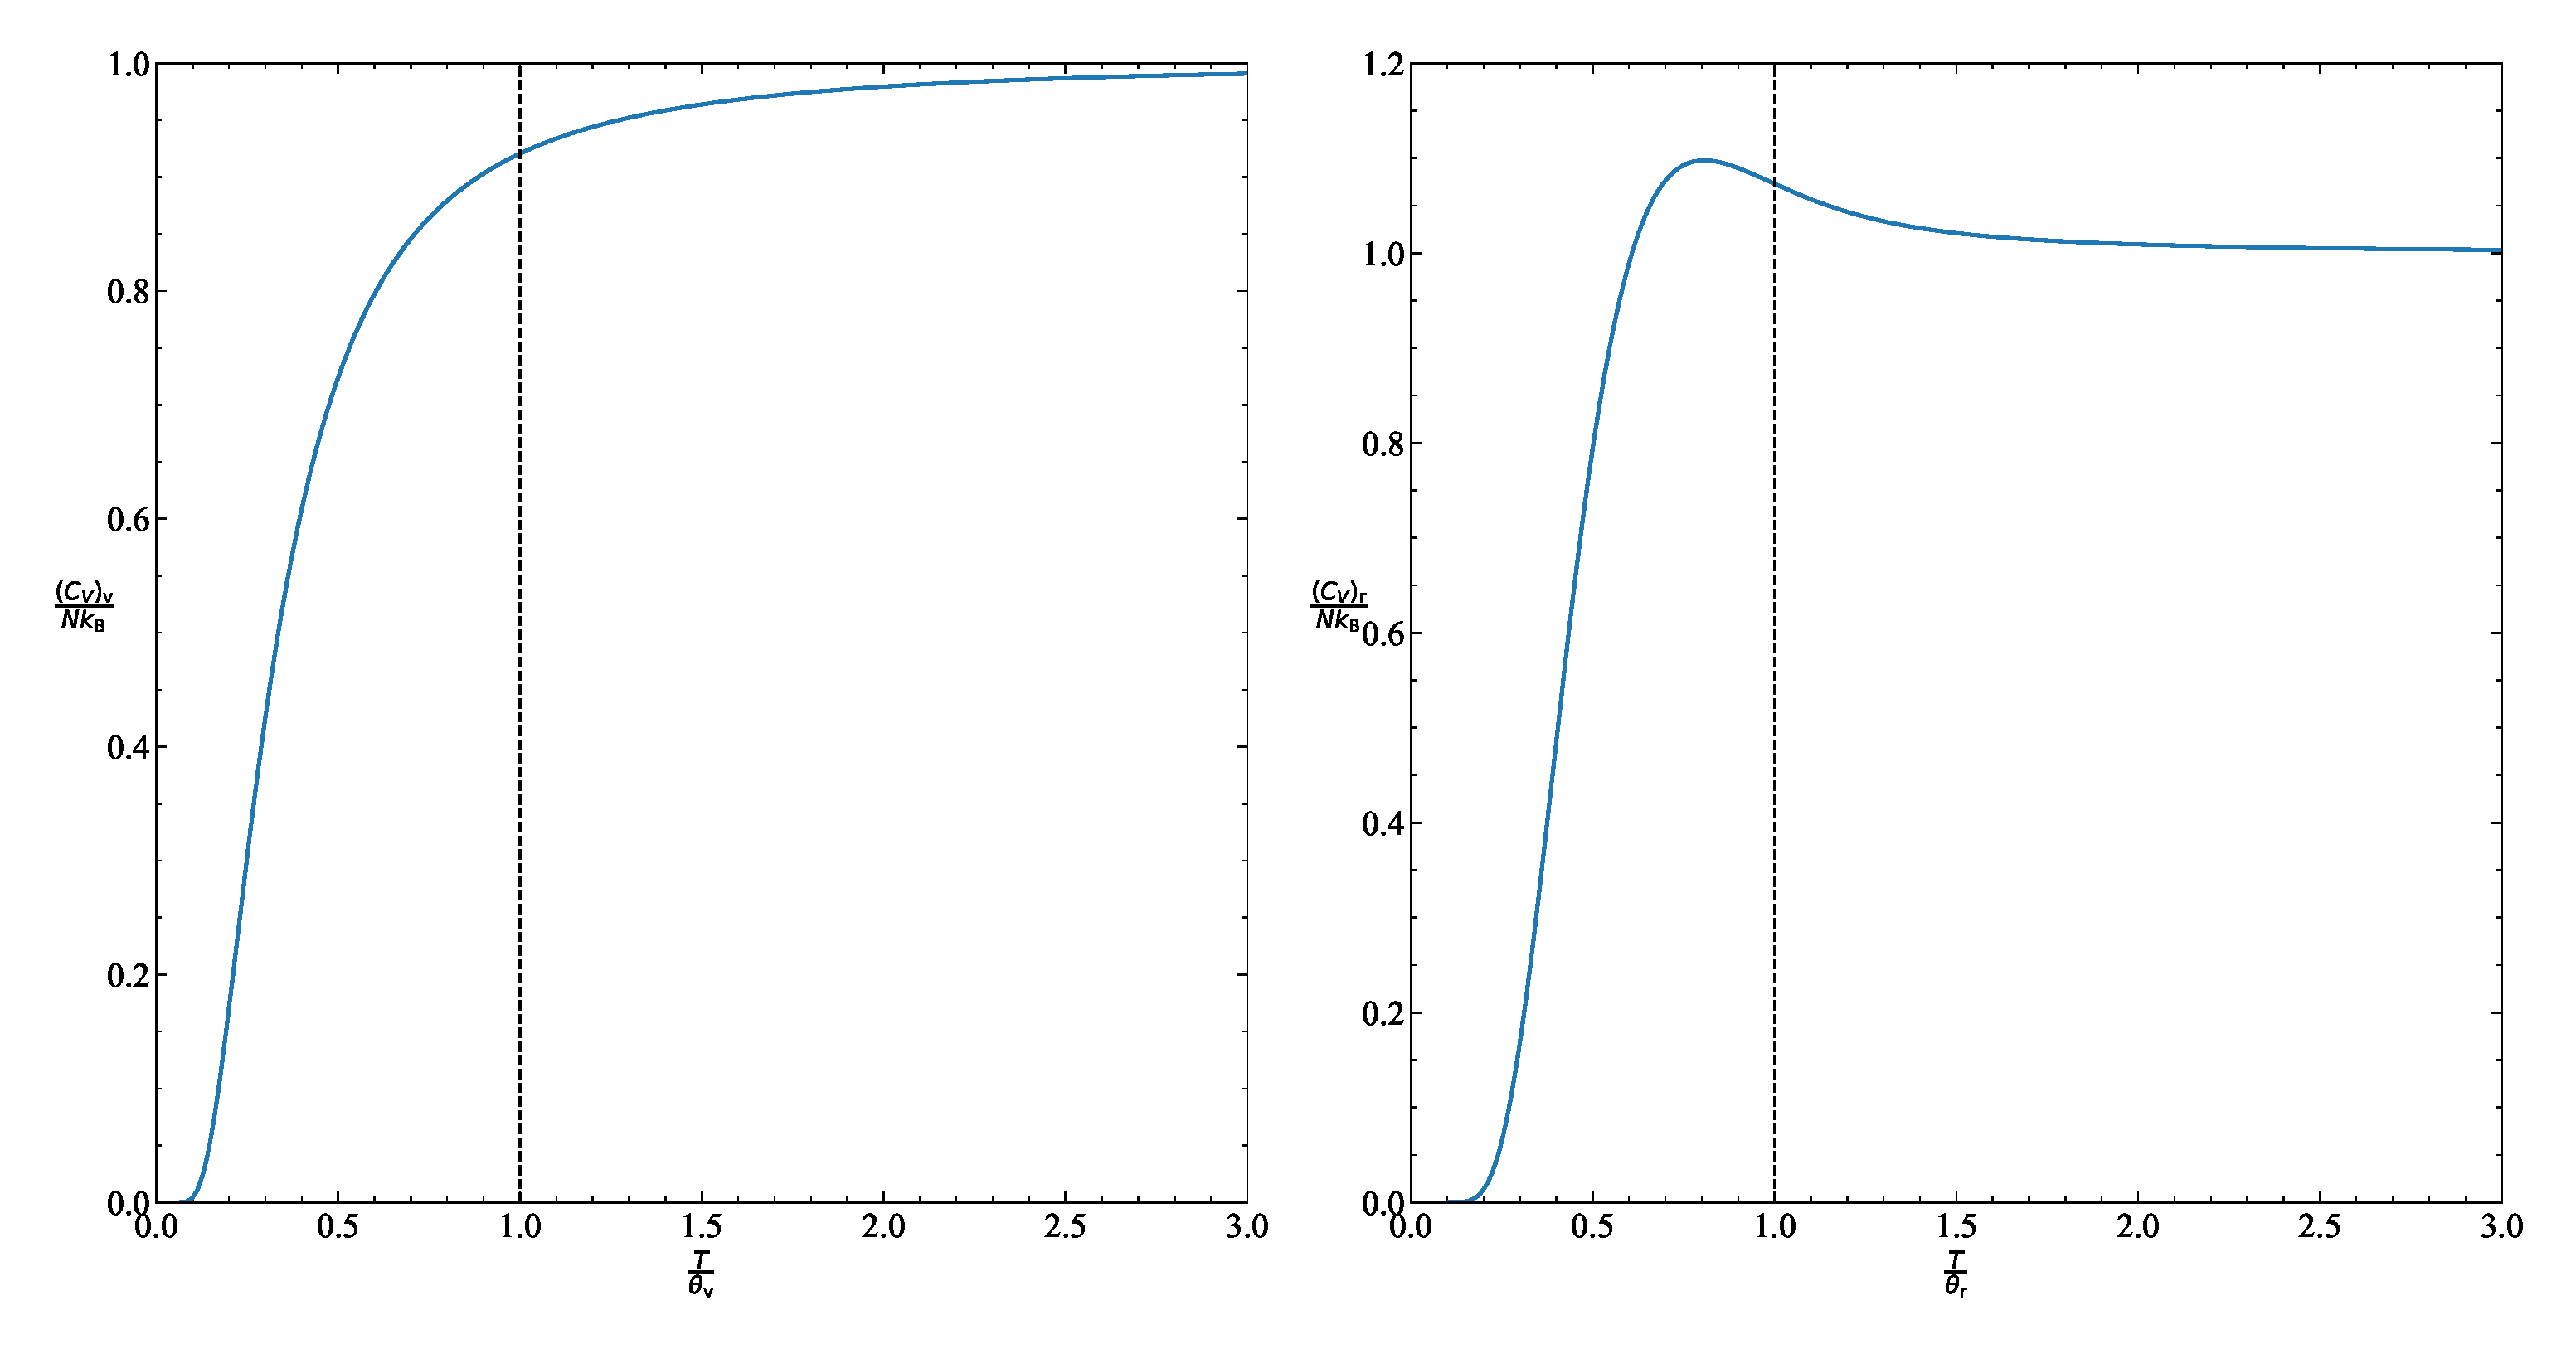
\includegraphics[width=\textwidth]{../../Figure/热统/正则系综的若干应用/双原子振转热容示意图.eps}
    \caption{左图展示了振动热容随温度的变化规律，右图展示了转动热容随温度的变化}
    \label{fig:双原子振转热容示意图}
\end{figure}
前文的极限分析暗示我们，振动热容和转动热容随温度的变化规律大体上是一致的，读者从上图中也能看出，两者整体上变化规律确实相差不大。但是，对于大多数双原子分子，它们的\(\theta_{\mathrm{v}}\)和\(\theta_{\mathrm{r}}\)有着巨大的数值差异。一般来说双原子分子的\(\theta_{\mathrm{v}}\)在\(10^3\mathrm{K}\)的量级，而\(\theta_{\mathrm{r}}\)仅在\(10\mathrm{K}\)乃至几开尔文的量级，也就是\(\theta_{\mathrm{r}}\ll\theta_{\mathrm{v}}\)。我们选取两个具体的\(\theta_{\mathrm{v}}\)和\(\theta_{\mathrm{r}}\)，画出热容随温度的变化曲线如图\ref{fig:双原子分子热容}所示。
\begin{figure}[H]
    \centering
    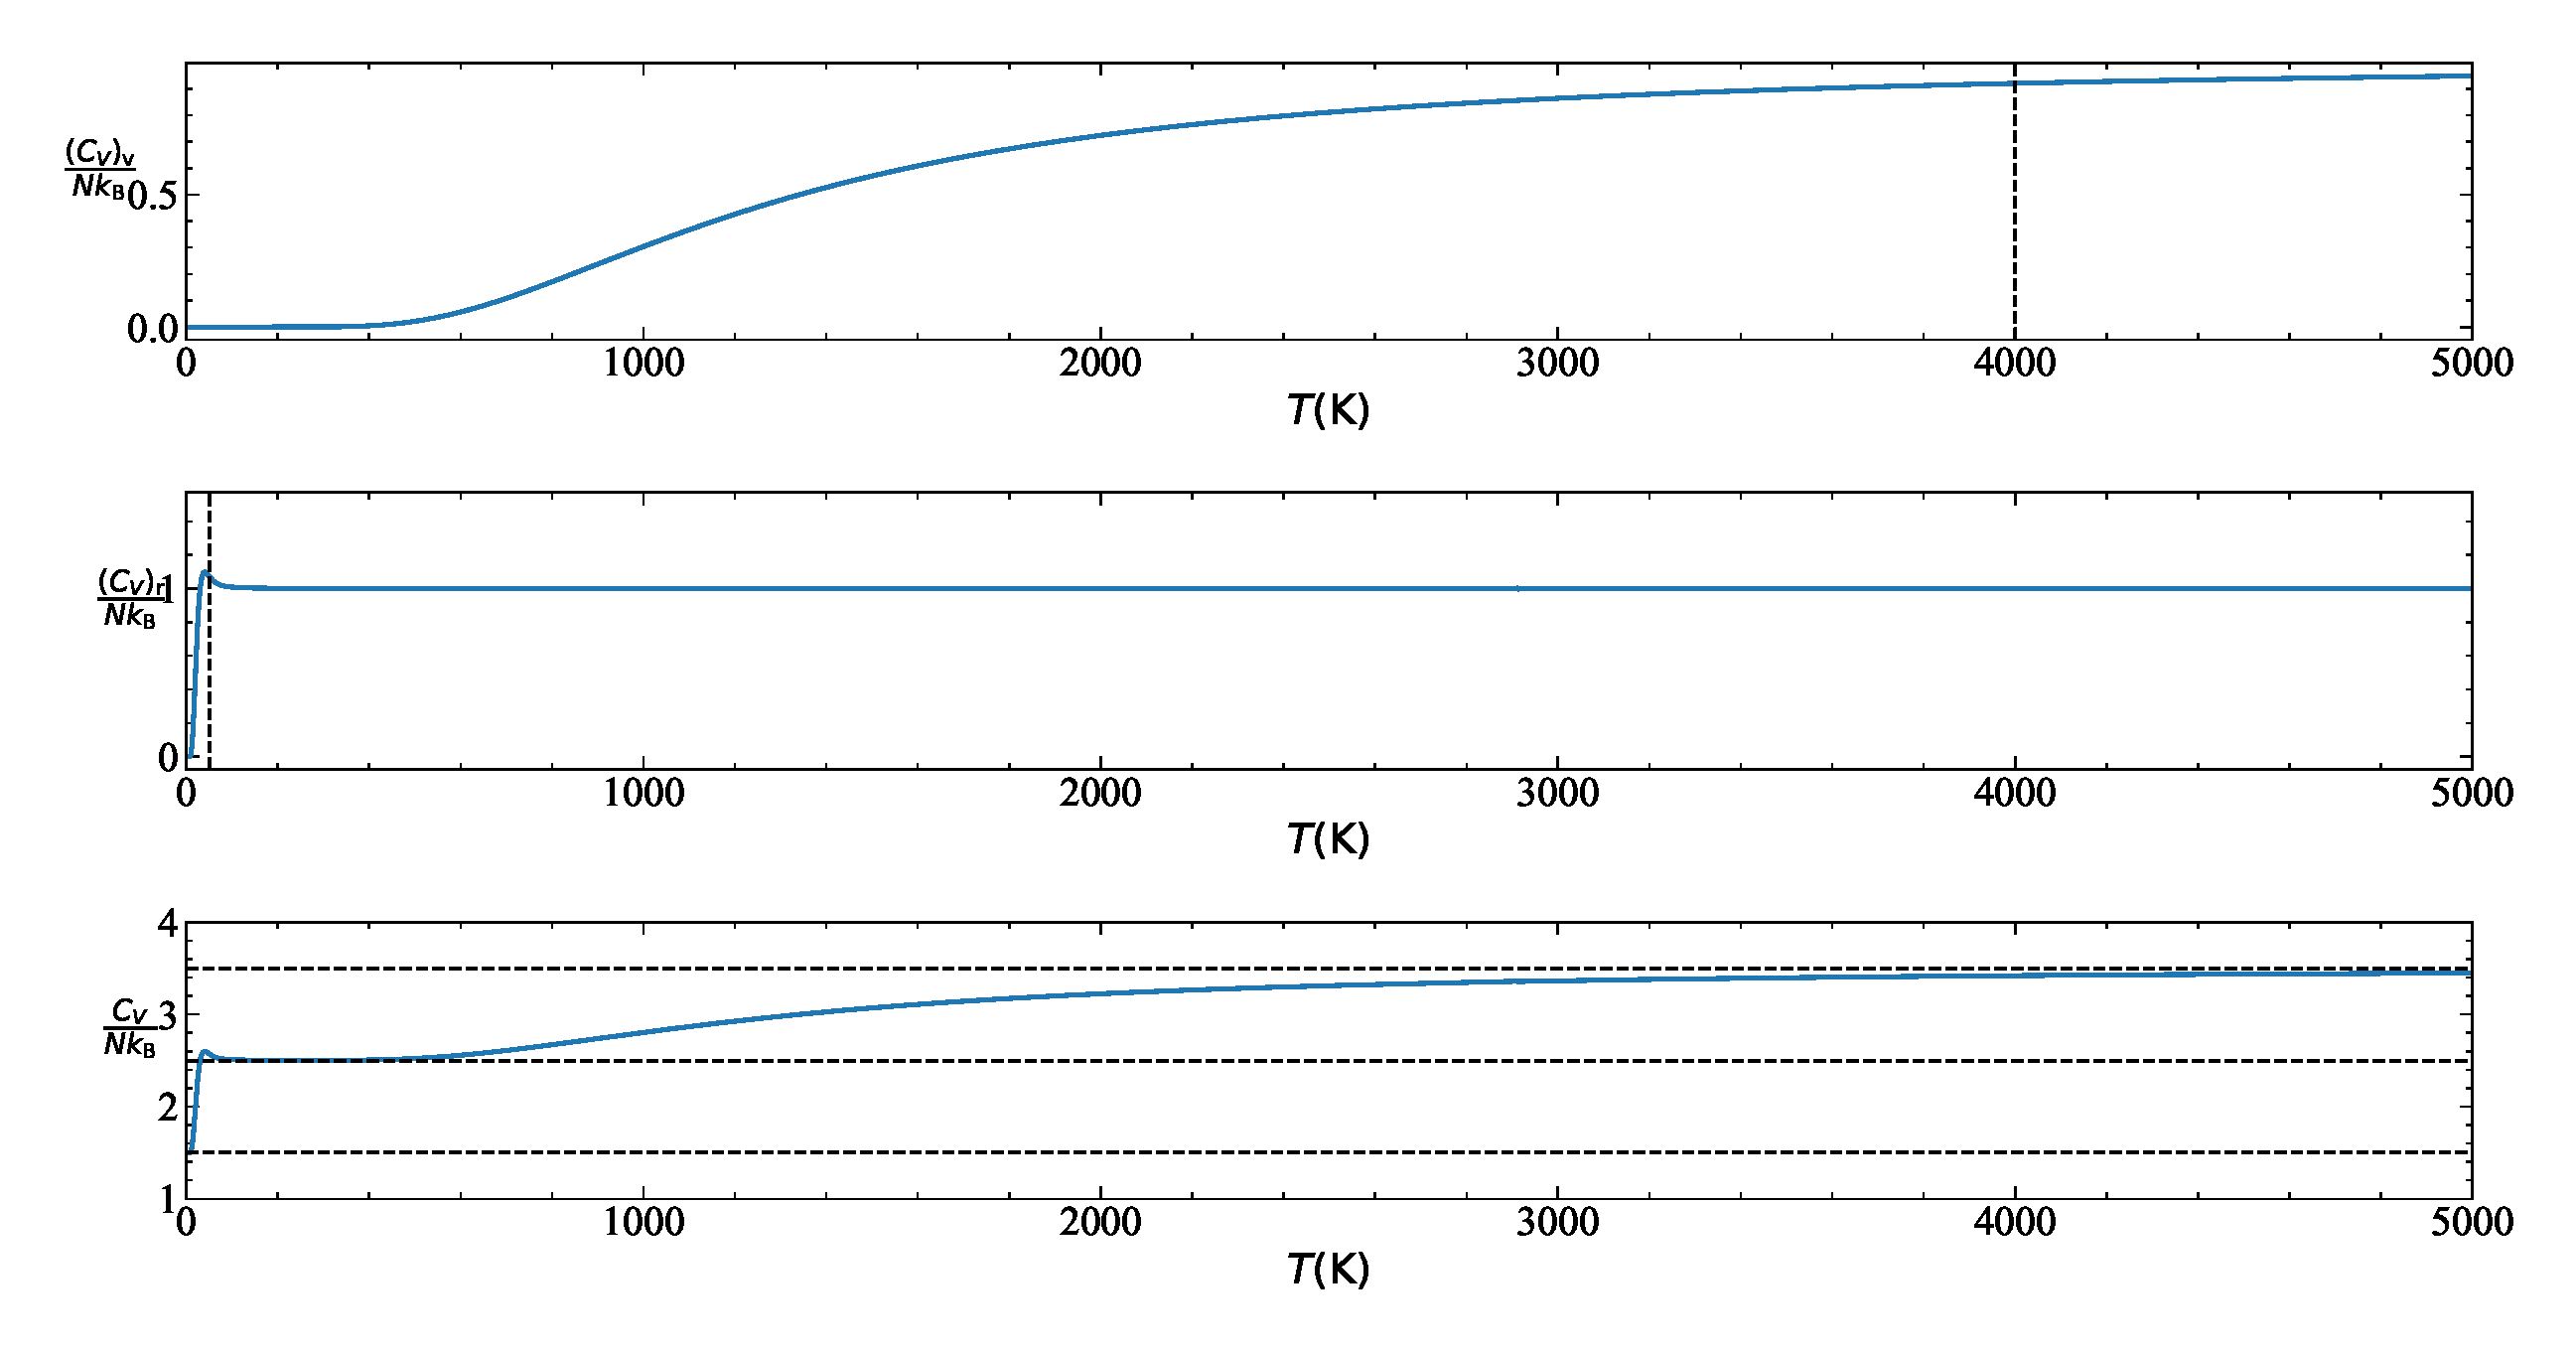
\includegraphics[width=\textwidth]{../../Figure/热统/正则系综的若干应用/双原子分子热容.eps}
    \caption{双原子分子的热容图像。第一幅图为振动热容，选择\(\theta_{\mathrm{v}}=4\times10^3\mathrm{K}\)，第二幅图为转动热容，选择\(\theta_{\mathrm{r}}=50\mathrm{K}\)，第三幅图为总热容。}
    \label{fig:双原子分子热容}
\end{figure}
可以看到，在一个温度尺度下比较振动热容和转动热容，它们看起来有着巨大差异。有意思的是，两个特征温度的巨大量级差距导致了如下现象。在温度远低于\(\theta_{\mathrm{r}}\)时，此时转动和振动都被“冻结”，因此气体热容为\(\frac{3}{2}N\k\)；随温度升高，转动被逐渐激发，当温度远大于\(\theta_{\mathrm{r}}\)而远小于\(\theta_{\mathrm{v}}\)时，转动被完全激发而振动还被“冻结”，因此热容是\(\frac{5}{2}N\k\)；随着温度继续升高，转动和振动都被激发，热容为\(\frac{7}{2}N\k\)。这正是热学课程所展示的只有量子力学才能解释的双原子气体分子热容平台效应，图\ref{fig:双原子分子热容}的第三幅图形象地展示了这一点。室温恰好处在远大于\(\theta_{\mathrm{r}}\)远小于\(\theta_{\mathrm{v}}\)这个区间，因此测得的许多双原子分子热容为\(\frac{5}{2}N\k\)，而且室温附近，可以认为热容几乎不变。

在本节的最后我们简单说明一下双原子分子振动和转动的动力学基础。对双原子分子的最简单建模是将其视为两个质点，这两个质点即两个原子之间的相互作用显然只与两原子的距离有关，那么问题就变成了所熟知的两体问题。在经典力学中，我们知道两体问题可以转化成两个假想粒子的运动，分别称为质心粒子和相对粒子，前者代表质心的运动，后者代表两质点的相对运动。我们主要关注相对粒子在原子间相互作用势下的运动。读者算出相对粒子的哈密顿量\footnote{\(H=\frac{P_r^2}{2\mu}+V(r)+\frac{1}{2\mu r^2}\left(P_{\theta}^2+\frac{1}{\sin^2\theta}P_{\varphi}^2\right)\)其中\(\mu\)为约化质量}后不难发现，径向变量\(r\)和角向变量\((\theta,\varphi)\)是耦合的，我们无意在动力学上深入这个耦合问题，因为对于我们所考虑的体系，两者可以认为是非耦合的。两个原子之所以能形成分子，是因为它们的相互作用能在某处不妨记为\(r_{\mathrm{e}}\)，存在势能最低点，这是系统的平衡位形。两个原子束缚成一个分子那么两者的距离必然不会偏离\(r_{\mathrm{e}}\)过远，也就是说相对粒子的\(r\)在\(r_{\mathrm{e}}\)附近做微振动，这种振动被称为双原子分子的振动\footnote{显然这是一个单自由度的振动，所以振动配分函数对应单个谐振子而不是两个谐振子，读者不要误以为两个原子在振动就是两个谐振子了}。正因为\(r\)做微振动，因此我们可以认为\(\frac{1}{2\mu r^2}\approx\frac{1}{2\mu r_{\mathrm{e}}^2}\)，其中\(\mu r_{\mathrm{e}}^2\)就是转动能级中的转动惯量\(I\)，这样相对粒子的角向运动就是一个半径为\(r_{\mathrm{e}}\)的球面上的运动，这种运动被称为双原子分子的转动\footnote{从相对粒子的视角退回两个原子的视角，这种转动就是一个刚性转子绕其质心的转动。利用经典力学的结论读者很容易想到，因为角动量守恒，刚性转子的转动实际上是平面转动。这会得出只有一个转动自由度的结论，但能量均分定理断定转动有两个自由度。这其中的矛盾在于角动量守恒是结论而不是约束，改变初始条件就会改变转子运动的平面，因此转子仍然是在一个三维空间中运动，有两个自由度}。我们的分析一直假定了经典力学视角，其实在量子力学中这种认识也是成立的，区别在于经典力学中跟运动相关的物理量都是连续的，而量子力学中振动能量是量子化的，角动量也是量子化的（这导致了转动能量的量子化）。关于双原子分子的动力学远不止这些，比如我们自始至终都没考虑电子的运动和两个原子是否相同，这些额外的动力学考量会导致新的统计物理计算，最终会产生怎样的修正这留给读者自行学习\footnote{关于双原子分子的量子化可以参考C.Cohen-Tannoudji《量子力学（第一卷）》，关于双原子分子的统计可以参考R.K.Pathria《统计力学》}。

\section{电磁辐射的统计理论}

到此为止，关于统计物理的实例讨论，大多都集中在经典理想气体这一熟悉的模型上，导出的结论也是在大家预料之中的，从结果来说没有给出超过热力学的内容。从本节开始我们的视角要扩展到更广阔的领域去，首先要处理的是一个颇具传奇色彩的内容——电磁辐射。这里所讨论的电磁辐射指的是恒温空窖中的平衡电磁辐射，历史上它有一个响当当的名字即黑体辐射，本节的第三小节将说明为什么它被称为黑体辐射。

任何物体都会发射电磁波，即热辐射。我们设想一个温度为\(T\)的大空窖，那么空窖会向其内部辐射电磁波，这些电磁波又被空窖吸收。如此辐射吸收平衡后，空窖内部的电磁波的内能和内能随电磁波频率的分布不再改变，我们称这种辐射为平衡辐射。这是我们对平衡电磁辐射的基础认识，热力学理论基于此已给出不少有益的结论。本节我们将从统计物理出发，讨论电磁辐射的各种热力学性质，主要是其内能密度和内能密度随频率的分布。

\subsection{谐振腔中的简正模式}
我们的统计从配分函数出发，那么首先就要知道电磁辐射的能级，或者说简单了解电磁场的量子态。在统计物理课程中这是无法讨论的，这个课题过于超前。不过电磁场相较于粒子系统有一个不同的地方在于，粒子系统只有在量子理论中是能量量子化的，电磁场在经典领域就有类似的“能量量子化”。更准确的说，封闭空间中的电磁场存在分立的定态解，这些定态解在时间上简谐变化而在空间中服从一定的方程，通过边界条件的限制\footnote{类似自由粒子的定态波函数，边界条件的限制导致了定态波函数的量子化。从计算的角度说，量子化往往来自边界条件的限制，经典粒子的运动是常微分方程无法用边界条件限制，量子理论中粒子的运动服从偏微分方程，就有了量子化的可能。}，这些解之间是分立的。这种定态解在电动力学课程中被称为电磁场的本征模式或简正模式，我们有必要简述一下电磁场的简正模式，因为我们的统计将依赖于它。
\begin{example}
    求解边长为\(L\)的立方谐振腔中的电磁波的简正模式，谐振腔的壁可视为理想导体。
    \begin{solution}
        所谓的谐振腔类似于三维盒子，只不过谐振腔中盛放的是电磁场，谐振腔的壁是理想导体保证了电磁场不外泄，数学上这将给出电磁场的本征方程的边界条件。谐振腔中可以认为是真空，显然这是一个无源区域，真空无源电磁场满足波动方程
        \begin{equation}
            \grad^2\bm{E}-\frac{1}{c^2}\pdv[2]{\bm{E}}{t}=0
        \end{equation}
        我们要求解的电磁波的简正模式实际上就是本征方程的解。为了得到本征方程，一般的做法要从分离变量开始，不过物理学家更喜欢从设试探解出发。具体来说，我们令电场随时间谐变，即假设\(\bm{E}(\bm{r},t)=\bm{E(\bm{r})}\mathrm{e}^{-\mathrm{i}\omega t}\)，代入上式可得
        \begin{equation}
            \grad^2\bm{E}+k^2\bm{E}=0\qquad k=\frac{\omega}{c}
        \end{equation}
        注意这个方程中的\(\bm{E}\)只是空间的函数，时间部分通过假设时间谐变被消去了。这是一个矢量方程，可以拆成三个分量方程，我们以\(E_{x}\)为例说明求解过程。显然\(E_{x}\)满足
        \begin{equation}
        \grad^2E_{x}+k^2E_{x}=0    
        \end{equation}
        这是大家比较熟悉的方程即亥姆霍兹方程，前文求解自由粒子的定态波函数时定态波函数也满足这一形式的方程，对它的分离变量不再赘述。设\(E_{x}=X(x)Y(y)Z(z)\)则
        \begin{equation}
            \begin{cases}
                \displaystyle \dv[2]{X}{x}+k_1^2x^2=0\qquad \eval{\dv{X}{x}}_{0}=\eval{\dv{X}{x}}_{L}=0 \\
                \displaystyle \displaystyle \dv[2]{Y}{y}+k_2^2y^2=0\qquad Y(0)=Y(L)=0 \\
                \displaystyle \displaystyle \dv[2]{Z}{z}+k_3^2z^2=0\qquad Z(0)=Z(L)=0
            \end{cases}
        \end{equation}
        其中\(k_1,k_2,k_3\)为三个本征值，它们满足\(k_1^2+k_2^2+k_3^2=k^2=\frac{\omega^2}{c^2}\)。本征方程的边界条件会在电动力学课程中导出，此处我们直接使用。满足这样边界条件的本征方程的解是很容易给出的，即
        \begin{equation}
            E_x=A_1\cos k_1x\sin k_2y\sin k_3z\qquad k_1=\frac{m\pi}{L}\quad k_2=\frac{n\pi}{L}\quad k_3=\frac{p\pi}{L}
        \end{equation}
        标记本征值的三个数字\(m,n,p\)均为非负整数。数学上本征方程的系数是无关紧要的，物理上却不一定。我们先保留这一系数，后文会说明它的用处。仿照类似的方法，可以求出另外两个分量\footnote{不难想到，三个分量每个分量对应三个本征值，实际上我们会得到九个本征值，之所以最终只出现三个本征值是因为电场要满足无散条件\(\div \bm{E}=0\)，读者学习电动力学课程时可以自行验证}
        \begin{equation}
            \begin{split}
                &E_x=A_1\cos k_1x\sin k_2y\sin k_3z \\
                &E_y=A_2\sin k_1x\cos k_2y\sin k_3z \\
                &E_z=A_3\sin k_1x\sin k_2y\cos k_3z
            \end{split}
        \end{equation}
        这样的解不一定是物理解，谐振腔中没有电荷，电场要满足\(\div \bm{E}=0\)，将上述解带入可得系数之间的关系
        \begin{equation}
            k_1A_1+k_2A_2+k_3A_3=0
        \end{equation}
        也就是说电场的三个分量的振幅\footnote{称其为振幅是不怎么合适的，因为本征解是驻波而不是行波，各点振幅不同，实际上它就是三个分量为了满足无散条件而引入的常数因子}是不独立的，它们要满足一个约束，由此可得对于一组\((m,n,p)\)，有两个独立的本征解。这一事实也可以这么理解\footnote{后文我们将电磁波视作光子，这一事实的理解方式就是光子有两个自旋取值}，电磁场是横波，有两种偏振方向。这样的本征解就是谐振腔中电磁场的简正模式。显然简正模式是分立的，此外简正模式没有数量限制，有无穷个简正模式。

        这一份粗略的教程并不试图让读者完全掌握谐振腔中电磁场的简正模式的全部特点，实际上我们求解的方程和所使用的边界条件都是从电动力学课程借用的，此处并没有详细说明。类似自由粒子的定态波函数，读者无需在意简正模式的具体表达式，只需知道，一组\((m,n,p)\)即一组\(k_1=\frac{m\pi}{L}, k_2=\frac{n\pi}{L}, k_3=\frac{p\pi}{L}\)给出两个简正模式，它们的波矢大小为\(k=\sqrt{k_1^2+k_2^2+k_3^2}\)，频率为\(\omega=ck\)。
    \end{solution}
\end{example}
从现在起，我们认为空窖就是这样一个边长为\(L\)的谐振腔，以利用我们求出来的各简正模式。简正模式之所以重要，是因为电动力学表明，谐振腔中电磁波的能量可以表示成一堆谐振子的能量和\footnote{后文我们会证明对于耦合谐振子系统，它的能量可以表示一堆谐振子的能量和，谐振子的频率正是耦合系统的简正频率。谐振腔中的电磁场的能量也有这种表示，读者可参考朗道《场论》第52节}，而每个谐振子都对应一个简正模式，其频率正是该简正模式的频率。学过量子力学的读者应该有感触，量子理论不是凭空而来的，它往往建立在经典理论的基础上\footnote{这就是所谓的“量子化”，从还原论的角度，世界上只有经典化而没有量子化，但受限于我们无法直接感知微观世界，量子理论往往都建立在经典理论的基础上}。量子化电磁场后，电磁场的能量也能表示为一堆谐振子的能量和，只是谐振子的能量是量子化的。所以我们关注的电磁辐射的能级，就是这一堆谐振子的能级，也就是我们可以认为平衡辐射就是谐振子构成的系统，因为有无穷个简正模式，所以平衡辐射系统有无穷个谐振子。这样的系统有确定的体积和温度，而粒子数是无穷，它能否使用正则系综的手段处理呢？我们无意深究，在课程中我们承认它是合理的，因为统计结论与实验高度相符。

最后，为了写出配分函数，我们要明确这些谐振子是否独立以及它们是否可分辨。各谐振子肯定是独立的，因为电磁场的能量是各谐振子的能量和，不包含各谐振子的相互作用。各谐振子也是可分辨的，因为每个谐振子都对应一个简正模式。简正模式类似定态\footnote{实际上在后文的巨正则系综部分，我们会把简正模式看成光子的量子态，不过在此处，请读者还是把简正模式理解成谐振子}，我们可以用四个“量子数”确定一个简正模式，其中三个为\((m,n,p)\)，剩下一个确定独立的两个简正模式，简正模式本身是可分辨的。我们可以给简正模式编上编号也就是可以给这些谐振子编号，所以谐振子是可分辨的。综上所述，平衡辐射就是一个由谐振子构成的玻尔兹曼系统，它的统计思路是简洁明了的。
\subsection{斯特藩-玻尔兹曼常量}
谐振子的单粒子配分函数是
\begin{equation}
    Z_1=\mathrm{e}^{-\frac{1}{2}\beta\hbar\omega}\frac{1}{1-\mathrm{e}^{-\beta\hbar\omega}}
\end{equation}
对于平衡辐射，各谐振子的频率即电磁波的简正频率不尽相同，我们不能简单把系统的配分函数写成上式的高次幂，要采用原始形式，即各谐振子的单粒子配分函数之积。对于配分函数的对数，其等于单粒子配分函数对数的和，即
\begin{equation}\label{eq:平衡辐射配分函数}
    \ln Z=\sum_{\text{所有模式}}\left[-\frac{1}{2}\beta\hbar\omega-\ln(1-\mathrm{e}^{-\beta\hbar\omega})\right]
\end{equation}
由此得到平衡辐射的内能为
\begin{equation}
    U=-\pdv{\ln Z}{\beta}=\sum_{\text{所有模式}}\left(\frac{1}{2}\hbar\omega+\frac{\hbar\omega}{\mathrm{e}^{\beta\hbar\omega}-1}\right)
\end{equation}

解析地计算这个求和是不可能的，因为这个求和类似\footnote{实际上此处的情况比计算自由粒子的单粒子配分函数更加糟糕，在那里，因为待求和函数是非耦合的，我们可以化简求和，对一个更简单的求和积分近似（我们没有具体讲述这一做法，因为意义不大），这里因为带求和函数的复杂性，我们甚至无法化简}自由粒子的单粒子配分函数，模式的离散性阻碍了我们的计算。解决方法相信读者也不难想到，求和不行积分近似，我们先凭感觉写出上式的积分近似式，接着再讨论这一近似所需的条件。经验告诉我们，我们需要引入一个叫简正模式密度的物理量，即
\begin{equation}
    U=\int_0^{\infty}\left(\frac{1}{2}\hbar\omega+\frac{\hbar\omega}{\mathrm{e}^{\beta\hbar\omega}-1}\right)g(\omega)\dd \omega
\end{equation}
其中\(g(\omega)\dd \omega\)表示电磁波的频率在\(\omega\sim\omega+\dd\omega\)范围内的模式数\footnote{类似于代数方程的重根算不同的根，我们可以说简正模式和简正频率是一一对应的，我们的统计根本不关心简正模式是什么，重要的是简正频率，所以\(g(\omega)\dd\omega\)最准确的理解是在\(\omega\sim\omega+\dd\omega\)范围内的简正频率的个数，而这些简正频率的值都是\(\omega\)}。因为前文求出的简正模式是用\((k_1,k_2,k_3)\)标记的，我们先计算\(g(k)\dd k\)，它表示波矢大小在\(k\sim k+\dd k\)范围内的模式数
\begin{equation}
    g(k)\dd k=2\frac{\frac{1}{8}4\pi k^2\dd k}{\left(\frac{\pi}{L}\right)^3}=\frac{Vk^2}{\pi^2}\dd k
\end{equation}
上式中的因子2是因为一个确定的\((k_1,k_2,k_3)\)对应两个简正模式。由色散关系\(\omega=ck\)可得\(\dd\omega=c\dd k\)，因此
\begin{equation}
    g(\omega)\dd\omega=g(k)\dd k=\frac{V}{\pi^2}\frac{\omega^2}{c^2}\frac{\dd\omega}{c}=\frac{V\omega^2}{\pi^2c^3}\dd\omega
\end{equation}
由此可得内能的表达式为
\begin{equation}\label{eq:平衡辐射内能}
    U=\int_0^{\infty}\left(\frac{1}{2}\hbar\omega+\frac{\hbar\omega}{\mathrm{e}^{\beta\hbar\omega}-1}\right)\frac{V\omega^2}{\pi^2c^3}\dd\omega
\end{equation}

不知读者是否有感觉，这里的数学处理和计算自由粒子的单粒子配分函数一模一样，只是物理解释不同。计算单粒子配分函数时待求和函数比较简单，因此可以给出一个相对简洁的近似条件，这里的求和函数比较复杂，近似条件不易导出，我们给出一个略显“耍赖”的条件即\(V\to\infty\)。这个条件也称为热力学极限，前文我们提过到\(N\to\infty\)是热力学极限，一般来说，热力学极限指的是粒子数和体积趋于无穷而粒子数密度保持有限。在热力学极限下，很显然\(\bm{k}\text{空间}\)中表示简正模式的格点\footnote{在计算单自由粒子配分函数时我们也可以取热力学极限，这样\(\bm{k}\text{空间}\)中表示量子态的格点会“连在一起”，那么求和也将变成积分。之所以没这么做一方面是因为我们可以给出更好的近似条件，另一方面热力学极限不会改变分子数密度，经典理想气体必须满足非简并条件，热力学极限对此没有任何帮助}会“连在一起”，简正模式变成连续的，因此用积分表示求和完全可以\footnote{把求和变成积分需要待求和函数随求和变量变化缓慢，那么我们可以限制待求和函数这就是所谓的高温条件，或者也可以限制求和变量即热力学极限。后者随略显耍赖，但它不需要考虑待求和函数的性质，有很强的推广性，读者学习量子场论时还会接触到这种技巧}。考虑到实际系统的体积总是有限的，所以最终我们的理论要接受实践的检验，能符合实验的理论总是一个不差的理论。

现在我们来着手计算平衡辐射的内能\eqref{eq:平衡辐射内能}。不难看出内能可以分成两项，第一项
\begin{equation}
    U_0=\sum_{\text{所有模式}}\frac{1}{2}\hbar\omega\quad \text{或}\quad U_0=\int_0^{\infty}\frac{1}{2}\hbar\omega\frac{V\omega^2}{\pi^2c^3}\dd\omega
\end{equation}
无论是求和形式还是积分形式它都是发散的，因为这表示所有简正模式的零点能的总和。对于我们的统计物理课程，这个发散项可以直接舍去，可以认为它是能量的零点不具有观测效应。对于第二项，简单地把体积移到等号左边即可得到内能密度的表达式
\begin{equation}\label{eq:平衡辐射的内能密度}
    u=\frac{U}{V}=\int_0^{\infty}\frac{\hbar}{\pi^2c^3}\frac{\omega^3}{\mathrm{e}^{\beta\hbar\omega}-1}\dd\omega\xlongequal{\beta\hbar\omega=x}\frac{\hbar}{\pi^2c^3}\frac{1}{(\beta\hbar)^4}\int_0^{\infty}\frac{x^3}{\mathrm{e}^x-1}\dd x=\frac{\pi^2\k^4}{15\hbar^3c^3}T^4
\end{equation}
上式用到了积分公式\footnote{\(\displaystyle \zeta(s)=\sum_{n=1}^{\infty}\frac{1}{n^s}\)即黎曼函数，\(\zeta(4)=\frac{\pi^4}{90}\)}
\begin{equation}
    \int_0^{\infty}\frac{x^n}{\mathrm{e}^x-1}\dd x=\zeta(n+1)\Gamma(n+1)
\end{equation}
取\(n=3\)即得\(\int_0^{\infty}\frac{x^3}{\mathrm{e}^x-1}\dd x=\frac{\pi^4}{15}\)，这个积分不需要读者记忆，可以查阅特殊积分表获得。将这个公式与热力学中的内能公式\(u=\frac{4\sigma}{c}T^4\)比较可得斯特藩-玻尔兹曼常量的值为
\begin{equation}
    \sigma=\frac{\pi^2\k^4}{60\hbar^3c^2}
\end{equation}
在热力学理论中，斯特藩-玻尔兹曼常量只能由实验拟合得到，在普朗克发表他划时代的黑体分布论文后，这个常量可以由更基本的物理学常数表示出来。有意思的是，这个常量所含的三个物理学常数分别代表着热理论、量子理论和电磁理论，黑体辐射作为各个物理学科的交汇，能敲开现代物理的大门是理所应当的。



\subsection{黑体分布}
除了内能密度，平衡辐射还有一个更重要的物理量即内能密度随频率的分布，常被称为谱能量密度\(u_{\omega}\)。其定义如此下，\(u_{\omega}\dd \omega\)表示频率在\(\omega\sim\omega+\dd\omega\)范围内的电磁波的能量密度，那么显然有
\begin{equation}
    u=\int_0^{\infty}u_{\omega}\dd \omega
\end{equation}
这是一个类似态密度的概念。此外还可以定义\(u_{\lambda}\dd \lambda\)，表示波长在\(\lambda\sim\lambda+\dd\lambda\)范围内的电磁波的能量密度，两者的关系\footnote{同样注意\(u_{\omega}\)和\(u_{\lambda}\)是两个函数。因为\(\omega=\frac{2\pi c}{\lambda}\)，所以\(\dd\omega\)与\(\dd\lambda\)异号，我们对谱能量密度的积分总是从0积到正无穷，或者说我们不在意范围的方向，因此两个谱能量密度的关系式中对微分要加绝对值}为\(u_{\lambda}\abs{\dd\lambda}=u_{\omega}\abs{\dd\omega}\)。根据这个定义，谱能量密度的表达式已是呼之欲出，但我们要先停下来简要说明一下平衡辐射和黑体辐射的关系。
\begin{example}
    由基尔霍夫定律给出平衡辐射和黑体辐射的关系。
    \begin{solution}
        物体除了自身产生热辐射，还会反射照射到其表面上的热辐射，也就是说会吸收热辐射，在本例题中我们考查空窖的内表面上某个面积微元的热辐射和对热辐射的吸收。照射到面积微元上的热辐射即平衡辐射的辐射通量密度\(J=\frac{1}{4}uc\)，面积微元会吸收这个热辐射，我们没有理由认为微元对不同波长的电磁波的吸收是相同的，因此我们在一定的波长范围内考虑。这样照射到面积微元上的热辐射是\(\frac{1}{4}u_{\lambda}\dd\lambda c\)，定义表面的辐射吸收率为\(\alpha_{\lambda}\)，这是一个无量纲量，表示对某一波长的吸收率，那么微元吸收的热辐射为
        \begin{equation}
            \left(\frac{1}{4}u_{\lambda}\dd\lambda c\right)\alpha_{\lambda}
        \end{equation}
        假设面积微元的热辐射为\(e_{\lambda}\dd\lambda\)，那么平衡时，吸收与辐射必然相当，即
        \begin{equation}
            \frac{e_{\lambda}}{\alpha_{\lambda}}=\frac{c}{4}u_{\lambda}
        \end{equation}
        上式表明空窖表面的热辐射能力与热吸收能力\footnote{注意\(e_{\lambda}\)和\(\alpha_{\lambda}\)的量纲是不一致的，前者表示单位波长单位面积的辐射功率，请读者仔细分辨这些物理量的量纲}成正比，又因为空窖的材料是任意的，我们可以断言在一定的温度下，若某物体对某一波长是良好的吸收体，那必定也是良好的辐射体，这就是基尔霍夫定律。根据这个判断，假设一种材料，它对所有的波长都是全吸收，即\(\alpha_{\lambda}=1\)对所有的\(\lambda\)均成立，那么显然有
        \begin{equation}
            e_{\lambda}=\frac{c}{4}u_{\lambda}
        \end{equation}
        不难看出，这个物体的辐射和平衡辐射一模一样。我们称这种对所有波长全吸收的物体为绝对黑体，简称黑体，它的热辐射称为黑体辐射，那么黑体辐射就是平衡辐射。实践上更有意义的是黑体向外发出的辐射，而我们的理论一直在讨论封闭空窖中的平衡辐射，其原因就在于此。

        理想的黑体是不存在的，倘若在一个大空窖\footnote{空窖内表面已经预先涂上了吸光材料}的壁上凿一个小孔，外界照射到小孔上的电磁波在空窖内部不断被反射吸收，在离开小孔前往往已被完全吸收，因此可以近似认为小孔不反射任何电磁波，那么小孔就近似是一个黑体。根据基尔霍夫定律，小孔的热辐射是平衡辐射；另一方面，小孔很小以至于空窖内的平衡电磁辐射没有被破坏，从小孔露出来的电磁波确实是平衡辐射，这直接说明了黑体辐射就是平衡辐射。
    \end{solution}
\end{example}
基于这种认识，我们称平衡辐射的谱能量密度为黑体分布，由式\eqref{eq:平衡辐射的内能密度}不难得到黑体分布为
\begin{equation}
    u_{\omega}=\frac{\hbar}{\pi^2c^3}\frac{\omega^3}{\mathrm{e}^{\beta\hbar\omega}-1}
\end{equation}
采用波长作自变量，根据\(\omega=2\pi c/\lambda\)黑体分布也可以写成
\begin{equation}
    u_{\lambda}=u_{\omega}\abs{\dv{\omega}{\lambda}}=\frac{8\pi hc}{\lambda^5}\frac{1}{\mathrm{e}^{\beta hc/\lambda}-1}
\end{equation}
倘若不采用角频率而使用频率\footnote{历史上普朗克给出的黑体分布公式就是以频率为自变量}，根据\(\omega=2\pi\nu\)可得
\begin{equation}
    u_{\nu}=u_{\omega}\dv{\omega}{\nu}=\frac{8\pi h}{c^3}\frac{\nu^3}{\mathrm{e}^{\beta h\nu}-1}
\end{equation}
取长波极限即低频极限，那么\(\beta h\nu\ll 1\)即\(h\nu\ll\k T\)，上式近似为
\begin{equation}
    u_{\nu}\approx\frac{8\pi h}{c^3}\frac{\nu^3}{\beta h\nu}=\frac{8\pi\k T}{c^3}\nu^2
\end{equation}
上式没有出现普朗克常数，在普朗克提出黑体分布的正确公式前就被人们发现即瑞利-金斯公式\footnote{利用能量均分定理，认为每个简正模式贡献的内能为\(\k T\)，就能得到瑞利-金斯公式}。两者的区别可以看下图中的左图。
\begin{figure}[H]
    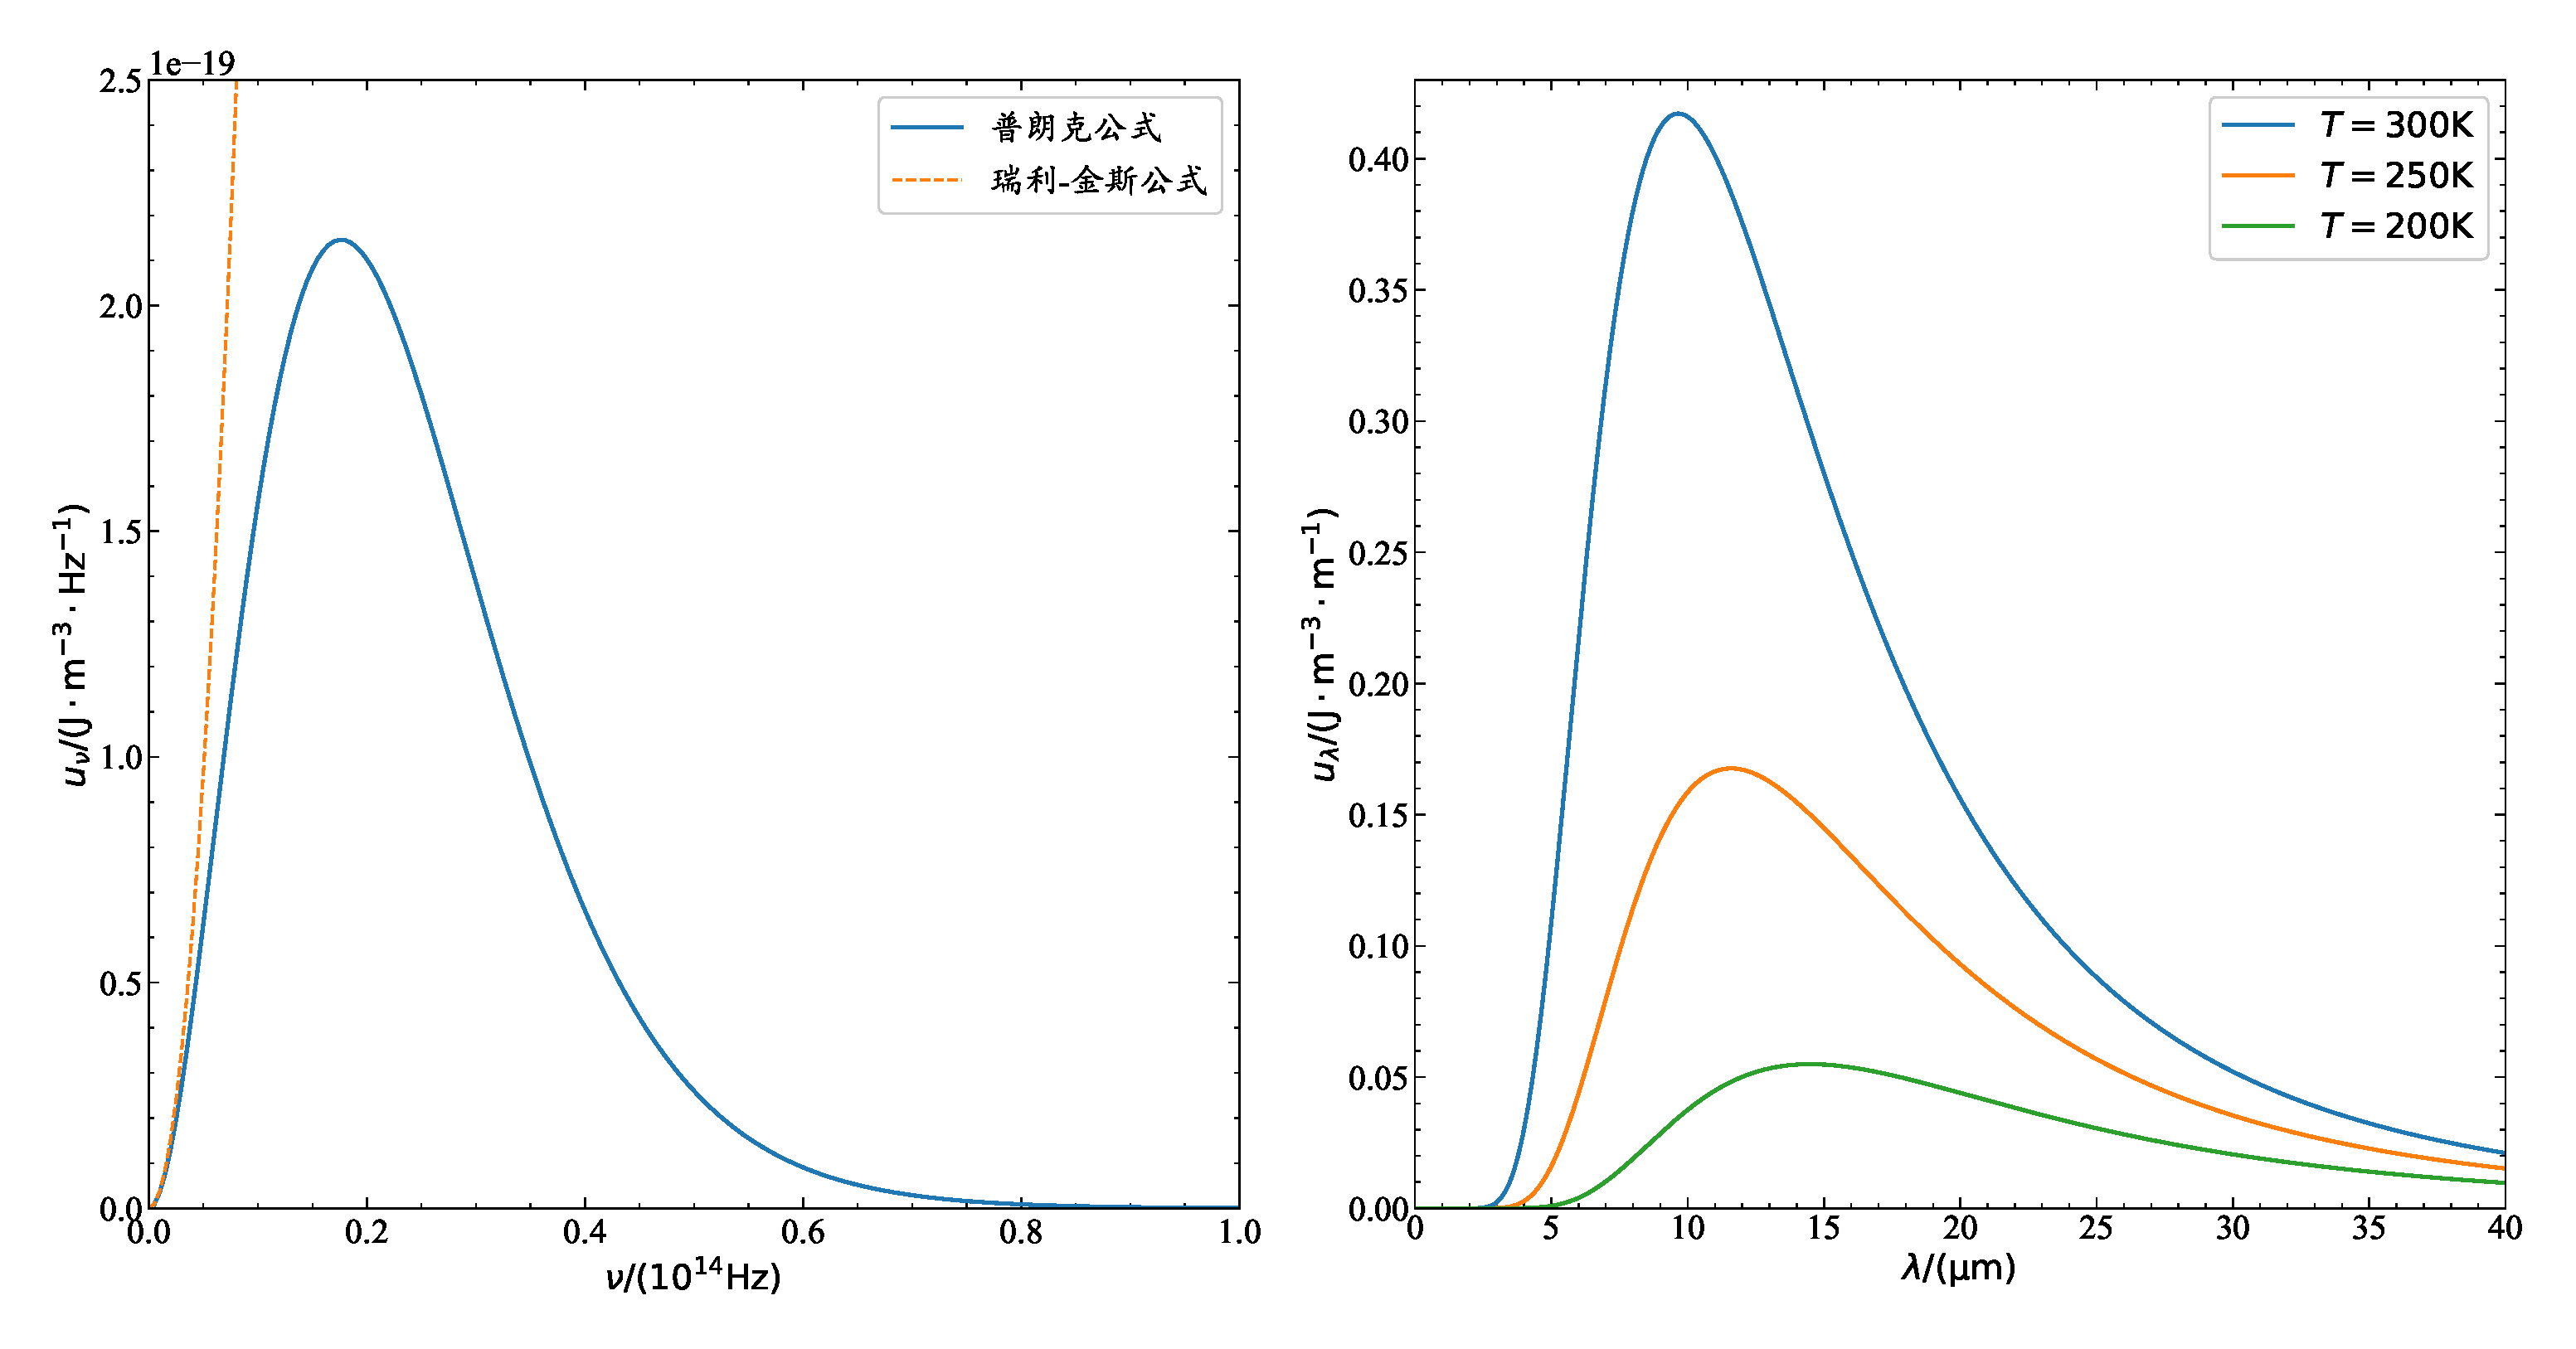
\includegraphics[width=\textwidth]{../../Figure/热统/正则系综的若干应用/黑体分布示意图.eps}
    \caption{从左图（\(T=300\mathrm{K}\)）中可以看到低频波段瑞利-金斯公式与普朗克公式符合较好而高频波段出现所谓的“紫外灾难”。从右图可以看出随着温度升高，最强辐射对应的波长逐渐变短。两图相比，\(T=300\mathrm{K}\)时两种形式的黑体分布（在适当的坐标刻度下）差别不大，但后文的分析将表明，它们的峰随温度的移动截然不同。}
\end{figure}
倘若认为瑞利-金斯公式在全波段成立，显然这个不断增长的谱能量密度会导致发散的内能密度，因为发散出现在高频部分，这被称为黑体辐射的“紫外灾难”。不过紫外灾难更像是一个激动人心的故事，紫外灾难这一说法在普朗克提出黑体分布十年之后才被提出，此时黑体分布早已被解决。而且普朗克本人也不认为能量均分定理是恒成立的，对他来说瑞利-金斯公式在高频段是必然不成立，那又何来灾难一说。

任何一个合理的分布，必然存在最大值。在普朗克之前，黑体分布的最大值对应的波长\(\lambda_{\text{max}}\)与温度的关系已被实验测得，即维恩位移定律\footnote{实际上基于热力学就可以推出维恩位移定律，而且形式比这里给出的形式更强，它限定了黑体分布的表达式，读者可以参考王竹溪先生的《热力学》第21节}，其表述为
\begin{equation}
    \lambda_{\text{max}}T=\text{常数}
\end{equation}
现在我们从黑体分布公式出发推导维恩位移定律，所需的数学运算仅是求导，即
\begin{equation}
    \dv{u_{\lambda}}{\lambda}=8\pi hc\left[-\frac{5\lambda^4(\mathrm{e}^{\beta hc/\lambda}-1)+\lambda^5\mathrm{e}^{\beta hc/\lambda}\left(-\frac{\beta hc}{\lambda^2}\right)}{\lambda^{10}(\mathrm{e}^{\beta hc/\lambda}-1)^2}\right]=0
\end{equation}
化简不难得到
\begin{equation}
    \frac{\beta hc}{\lambda}=5(1-\mathrm{e}^{-\beta hc/\lambda})
\end{equation}
这是一个关于\(\lambda\)的超越方程，但不难发现，\(\beta hc/\lambda\)作为一个整体出现，所以它的值是定值，因此有\(\lambda_{\text{max}}T\)是一个常数。数值计算给出上式的解为
\begin{equation}
    \frac{hc}{\lambda_{\text{max}}\k T}=4.96511
\end{equation}
维恩位移定律的另一种形式是\(\displaystyle \frac{\nu_{\text{max}}}{T}\)为常数，其推导过程类似
\begin{equation}
    \dv{u_{\nu}}{\nu}=\frac{8\pi h}{c^3}\frac{3\nu^2(\mathrm{e}^{\beta h\nu}-1)-\nu^3\mathrm{e}^{\beta h\nu}\beta h}{(\mathrm{e}^{\beta h\nu}-1)^2}=0
\end{equation}
化简后可以得到一个关于\(\beta h\nu\)的方程
\begin{equation}
    \beta h\nu=3(1-\mathrm{e}^{-\beta h\nu})
\end{equation}
数值计算给出的解为\footnote{注意\(\nu_{\text{max}}\neq\frac{c}{\lambda_{\text{max}}}\)，因为\(u_{\nu}\)和\(u_{\lambda}\)是不同的函数，不只是换元而已}
\begin{equation}
    \frac{h\nu_{\text{max}}}{\k T}=2.82144
\end{equation}
根据维恩位移定律可以简单估算，一个室温上下的黑体，它发出的辐射在\(10\mathrm{\mu m}\)附近最强，这位于电磁波谱的红外波段。常见的夜视仪或者热成像仪大多也叫红外热像仪，正是因为它主要利用热辐射中的红外电磁波。

普朗克提出的黑体分布公式\footnote{读者有兴趣可以阅读一下普朗克于1901年发表的论文《On the Law of Distribution of Energy in the Normal Spectrum》，感受一下普朗克是如何在量子力学和系综统计没有建立之前推出这个惊人的公式}有很大的实践意义，十九世纪的技术进步和工业界的新需求推动着人们对黑体辐射的研究，最终这一问题被普朗克解决，也推开了量子力学的大门。有意思的是，约半个世纪后人们在浩瀚星空中又发现了黑体分布的身影。美国新泽西州贝尔实验室的两位科学家偶然间发现天空中来自各个方向的似乎均匀的微波辐射，这个辐射的分布与温度为\(2.7\mathrm{K}\)的黑体分布\footnote{室温黑体对应\(10\mathrm{\mu m}\)，不难算出\(2.7\mathrm{K}\)的黑体对应\(1\mathrm{mm}\)，这对应电磁波谱的微波波段}高度吻合，后续的实验表明这个辐射的各向同性异常好，这一辐射被称为宇宙微波背景辐射，被认为是宇宙大爆炸理论的重要证据。不过笔者水平有限，不能在此展开详细分析，有兴趣的读者可查阅其他资料学习。

\subsection{平衡辐射的化学势}
前两节导出的结论都是热力学理论给不出来的，在本节的最后，我们用统计物理手段给出一个热力学中已有的结论。它是如此地重要以至于我们在这里要再次讲述。

由平衡辐射的配分函数\eqref{eq:平衡辐射配分函数}可得，其自由能为
\begin{equation}
    F=-\k T\sum_{\text{所有模式}}\left[-\frac{1}{2}\beta\hbar\omega-\ln(1-\mathrm{e}^{-\beta\hbar\omega})\right]
\end{equation}
略去自由能的零点并把求和变成积分，可得
\begin{equation}
    F=V\frac{\k T}{\pi^2c^3}\int_0^{\infty}\ln(1-\mathrm{e}^{-\frac{\hbar\omega}{\k T}})\omega^2\dd\omega
\end{equation}
无需计算上述积分的结果，我们可以直接得到\(F\propto V\)即
\begin{equation}
    p=-\left(\pdv{F}{V}\right)_{N,T}=-\frac{F}{V}
\end{equation}
由这一结果我们发现
\begin{equation}
    G=F+pV=0
\end{equation}
也就是说平衡辐射的吉布斯自由能为0。与吉布斯自由能绑定的另一个热力学量即化学势，它表示单粒子吉布斯自由能，显然平衡辐射的化学势\footnote{有读者可能认为平衡辐射的简正模式数为无穷，粒子数就是无穷，因此化学势为0。笔者认为这种想法并不恰当，因为平衡辐射的粒子数本身就没有定义，只是统计力学计算时把每个简正模式视作了一个谐振子}为0。后文在巨正则系综部分我们将把平衡辐射视作光子气体再次给出本节的结论，那里我们会用到光子的化学势为0，不过我们将从另一个角度说明这一事实。

\section{固体热容理论}
从本节开始，我们要学习如何计算固体或者说晶体的热容。在统计物理发展史上，这是继黑体分布之后量子力学和统计理论融合而产生的第二个成功理论。晶体中的原子因为强烈的相互作用只能在其平衡位置附近做微振动\footnote{在晶格动力学中原子做微振动被称为间谐近似，对于我们讨论的热容理论，间谐近似是足够的。在别的理论里就可能要考虑原子振动的非简谐效应。容易想到当温度过高以致固体融化时，简谐近似显然就不合理了，换句话说我们认为在所考虑的温度下，晶体的微观整体结构不会改变，温度变化只是影响原子振动的强弱而不会导致原子之间解离}，我们关注的就是这一微振动，也就是说我们关注各原子微振动的能量而不是整个固体的能量。各原子构成一个整体而形成晶体，因此它们的微振动是相互耦合的，不可能是独立的，也就是我们要考虑相互作用能，这就为我们的统计带来了困难。

幸运的是，我们马上会证明，经典力学视角下，利用简正坐标，我们能把系统的能量写成各独立谐振子的能量和，各个独立谐振子的频率正是固体的简正频率。量子力学中，采用类似的方法我们也能证明系统的能量是独立谐振子的能量和，不过谐振子的能量已是量子化的。这意味着我们不再处理每个原子的振动，而是关注系统的简正模式。每一个简正模式都对应一个独立的谐振子，其频率正是该简正模式的频率。读者不难发现，我们的理论和平衡辐射的统计理论非常相似\footnote{这种相似启发我们提出类似光子的概念——声子，我们将在巨正则系综部分介绍它}，但是由于固体本身的复杂性，第一性地解析计算固体的简正频率是不可能的，因此我们往往采用两种近似模型，分别是爱因斯坦模型和德拜模型。我们的课程将从一个纯力学的观念出发，再过渡到对两个模型的具体求解。

\subsection{两个耦合谐振子的哈密顿量}

我们考虑如下图所示的两个耦合谐振子，这是一个足够简单却又不失代表性的例子。
\begin{figure}[H]
    \centering
    \includegraphics[width=0.8\textwidth]{./耦合谐振子示意图.pdf}
    \caption{}
\end{figure}
图中两个谐振子的质量均为\(m\)而三个弹簧的进度系数均为\(k\)，长虚线表示谐振子的平衡位置，我们选取谐振子偏离平衡位置的距离为广义坐标。假设谐振子位于平衡位置时所有的弹簧都位于原长，那么系统的拉氏量\footnote{注意\(\dot{x}_1^2\)实际上是\(\dot{x_1}^2\)即\(x_1\)对应的广义速度的平方。因为\LaTeX 的排版美观问题，把点加到了\(x\)的上方而不是\(x_1\)整体的上方，不要把它理解成了\(x\)导数的第一个分量。如果读者一定要这么理解，那么\(x=(x_1,x_2)\)也仅仅是一个二元有序数对，它不是矢量，只是我们这个例子中系统的位形空间恰好是\(\mathbb{R}^2\)导致它看起来像一个矢量}为
\begin{equation}\label{eq:广义坐标拉氏量}
    \begin{split}
        L&=\frac{1}{2}m\dot{x}_1^2+\frac{1}{2}m\dot{x}_2^2-\frac{1}{2}kx_1^2-\frac{1}{2}kx_2^2-\frac{1}{2}k(x_1-x_2)^2 \\
        &=\frac{1}{2}m\dot{x}_1^2+\frac{1}{2}m\dot{x}_2^2-kx_1^2-kx_2^2+kx_1x_2
    \end{split}
\end{equation}
勒让德变换后可得系统的哈密顿量为
\begin{equation}
    H=\frac{P_1^2}{2m}+\frac{P_2^2}{2m}+kx_1^2+kx_2^2-kx_1x_2
\end{equation}
其中\(P_1\)和\(P_2\)分别是\(x_1\)和\(x_2\)对应的广义动量。从拉氏量或者哈密顿量中我们可以明显看出两个谐振子的运动是耦合的，下面我们将证明如果采用简正坐标，那么系统的运动将变成两个独立谐振子的运动。

计算系统的简正坐标是一件程序化的事情，下面我们展示一下计算过程，熟悉的同学可以直接跳过。对于这个高度对称的系统，读者应该能猜出来两个简正坐标的意义，分别代表系统质心的运动和谐振子的相对运动。
\begin{example}
    计算该耦合谐振子系统的简正坐标。
    \begin{solution}
        我们先计算系统的惯性矩阵\(\mathbf{M}\)和刚度矩阵\(\mathbf{K}\)，因为这个系统的振动无论是否强烈都是谐振动，所以两个矩阵仅仅是拉氏量的二阶偏导\footnote{如果系统本身是非谐振动的，通过微振动条件近似成谐振动系统，比如小摆角的双摆，那么这两个矩阵是拉氏量的二阶偏导在平衡位置即所有广义坐标都为0时的值}
        \begin{equation}
            \mathbf{M}=\pdv[2]{L}{\dot{x}_i}{\dot{x}_j}=\mqty(m & 0 \\ 0 & m)\qquad\quad \mathbf{K}=-\pdv[2]{L}{x_i}{x_j}=\mqty(2k & -k \\ -k & 2k)
        \end{equation}
        刚度矩阵关于惯性矩阵的广义特征值就是系统的简正频率平方，即
        \begin{equation}
            \abs{\mathbf{K}-\mathbf{M}\omega^2}=\mdet{2k-m\omega^2 & -k \\ -k & 2k-m\omega^2}=\Big(2k-m\omega^2\Big)^2-k^2=0
        \end{equation}
        不难看出上述方程的两个解为\(\omega_1=\sqrt{\frac{k}{m}}\)和\(\omega_2=\sqrt{\frac{3k}{m}}\)，将这两个解带入特征方程\((\mathbf{K}-\mathbf{M}\omega^2)A=0\)可以得到两个特征向量\footnote{简正频率对应的特征向量采用广义归一化即\(A_i^{\mathrm{T}}\mathbf{M}A_j=\delta_{ij}\)，实际上在整个计算体系中，惯性矩阵\(\mathbf{M}\)都充当着单位矩阵的作用}
        \begin{equation}
            A_1=\frac{1}{\sqrt{2m}}\mqty(1\\1)\qquad\quad A_2=\frac{1}{\sqrt{2m}}\mqty(\admat{1\\-1})
        \end{equation}
        特征向量的组合就是广义坐标\footnote{这里的广义坐标指的是最初选取的比较自然的广义坐标，简正坐标本质也是广义坐标}和简正坐标之间的变换矩阵，即
        \begin{equation}\label{eq:广义坐标简正坐标变换}
            \mqty(x_1 \\ x_2)=\mqty(A_1& A_2)\mqty(\xi_1\\ \xi_2)=\mqty(\frac{1}{\sqrt{2m}} &\frac{1}{\sqrt{2m}} \\ \frac{1}{\sqrt{2m}} & -\frac{1}{\sqrt{2m}})\mqty(\xi_1\\ \xi_2)=\mqty(\frac{1}{\sqrt{2m}}\xi_1+\frac{1}{\sqrt{2m}}\xi_2 \\ \frac{1}{\sqrt{2m}}\xi_1-\frac{1}{\sqrt{2m}}\xi_2)
        \end{equation}
        将上式反解就可以得到简正坐标的表达式
        \begin{equation}
            \mqty(\xi_1\\ \xi_2)=\mqty(\frac{\sqrt{2m}}{2}(x_1+x_2)\\ \frac{\sqrt{2m}}{2}(x_1-x_2))
        \end{equation}
        不难看出，两个简正坐标确实一个代表质心的运动一个代表相对运动。
    \end{solution}
\end{example}

实际上并不需要求出简正坐标的表达式，将变换关系\eqref{eq:广义坐标简正坐标变换}带入拉氏量\eqref{eq:广义坐标拉氏量}化简后就能得到用简正坐标表示的拉氏量
\begin{equation}
    L=\frac{1}{2}\dot{\xi_1}^2-\frac{k}{2m}\xi_1^2+\frac{1}{2}\dot{\xi_2}^2-\frac{3k}{2m}\xi_2^2=\frac{1}{2}\dot{\xi_1}^2-\frac{1}{2}\omega_1^2\xi_1^2+\frac{1}{2}\dot{\xi_2}^2-\frac{1}{2}\omega_2^2\xi_2^2
\end{equation}
上式最后一步使用了简正频率的表达式。从拉氏量我们已能看出，两个简正坐标的运动是解耦的。对上式勒让德变换后就得到了用简正坐标表示的哈密顿量
\begin{equation}\label{eq:简正坐标哈密顿量}
    H=\frac{\eta_1^2}{2}+\frac{1}{2}\omega_1^2\xi_1^2+\frac{\eta_2^2}{2}+\frac{1}{2}\omega_2^2\xi_2^2
\end{equation}
其中\(\eta_1=\pdv{L}{\dot{\xi}_1}=\dot{\xi}_1,\eta_2=\pdv{L}{\dot{\xi}_2}=\dot{\xi}_2\)是简正坐标的广义动量。这一形式的哈密顿量读者不一定熟悉，常见的谐振子哈密顿量为\(H=\frac{P^2}{2m}+\frac{1}{2}m\omega^2x^2\)，倘若采用\(\xi=\sqrt{m}x\)为广义坐标，读者可以检验其哈密顿量正是
\begin{equation}
    H=\frac{\eta^2}{2}+\frac{1}{2}\omega^2\xi^2
\end{equation}
这和式\eqref{eq:简正坐标哈密顿量}形式完全相同，只是式\eqref{eq:简正坐标哈密顿量}表示两个谐振子，这两个谐振子的频率为系统的简正频率。

对于这个系统，量子力学会给出类似的结论，不过谐振子的能量是量子化的，即系统的能级为
\begin{equation}
    E_{n_1,n_2}=\left(n_1+\frac{1}{2}\right)\hbar\omega_1+\left(n_2+\frac{1}{2}\right)\hbar\omega_2
\end{equation}
这显然是两个独立谐振子的能量和，其中的两个频率正是系统的简正频率。对于我们的统计理论，重要的是系统的能量而不是粒子的能量，从这个角度来说，倘若我们考虑一个耦合谐振子系统的热性质，那么把它视为一堆孤立谐振子构成的系统，对我们的统计是必要的\footnote{读者应该能从这里感受的强烈的化归思想，系综统计可以方便地处理无相互作用系统，对于有相互作用系统，首先要想办法将其转化为无相互作用系统，不行的话再发展其他方法}。

\subsection{固体热容理论}
对于由\(N\)个原子构成的晶体，每个原子在空间中做微振动，那么系统一共有\(3N\)个振动自由度。根据上一小节的结论，这样一个耦合的谐振子系统，其能量为\(3N\)个独立谐振子的能量和，谐振子的频率\footnote{实际上也只有独立谐振子才有频率的概念，因为我们讨论的频率都是固有频率，一个耦合谐振子的固有频率是没有意义的}为系统的简正频率。因为简正频率和简正模式是一一对应的，所以这\(3N\)个谐振子对应\(3N\)个简正模式，也就是说一个简正模式对应一个谐振子。读者对这一观点应该不陌生，上一节我们处理平衡辐射时就采用了这一观点。显然这些谐振子是可分辨的，因为振动系统的简正模式表示所有振动自由度以相同频率振动的特解，自然是可分辨的。那么，固体系统也可以被看成是谐振子构成的玻尔兹曼系统。由此给出的配分函数和上一节的式\eqref{eq:平衡辐射配分函数}是完全相同的
\begin{equation}
    \ln Z=\sum_{\text{所有模式}}\left[-\frac{1}{2}\beta\hbar\omega-\ln(1-\mathrm{e}^{-\beta\hbar\omega})\right]
\end{equation}
对上式求导我们得到内能，再次求导得到热容，详细的计算过程已在前文推导双原子分子气体的振动热容时展示过，这里直接给出结果
\begin{equation}\label{eq:固体内能公式}
    U=\sum_{\text{所有模式}}\left(\frac{\hbar\omega}{2}+\frac{\hbar\omega}{\mathrm{e}^{\beta\hbar\omega}-1}\right)
\end{equation}
\begin{equation}\label{eq:固体热容公式}
    C_V=\sum_{\text{所有模式}}\k\left(\frac{\hbar\omega}{\k T}\right)^2\frac{\mathrm{e}^{\frac{\hbar\omega}{\k T}}}{\left(\mathrm{e}^{\frac{\hbar\omega}{\k T}}-1\right)^2}
\end{equation}
值得注意的是，这里的表达式虽说和上一节的表达式形式相同，但电磁辐射的简正模式没有个数限制，而固体系统的简正模式只有\(3N\)个，是有限的。此外，我们可以计算出电磁辐射的各简正频率，而现在讨论的固体，我们不可能从量子力学出发直接计算出其\(3N\)个简正频率。
\subsection{爱因斯坦模型}
正如前文所言，我们需要近似模型来得到这\(3N\)个简正频率。第一个近似模型由爱因斯坦提出，被称为爱因斯坦模型。爱因斯坦模型粗略地认为这\(3N\)个简正频率相同都是\(\omega_{\mathrm{E}}\)。这一观点等价于所有的振动自由度以同一个频率\(\omega_{\mathrm{E}}\)振动，这显然是不怎么合适的，不过作为历史上第一个量子版本的固体热容理论，爱因斯坦模型有其独特的历史地位。

在这一近似下，不难看出，热容为
\begin{equation}
    C_V=3N\k \left(\frac{\hbar\omega_{\mathrm{E}}}{\k T}\right)^2\frac{\mathrm{e}^{\frac{\hbar\omega_{\mathrm{E}}}{\k T}}}{\left(\mathrm{e}^{\frac{\hbar\omega_{\mathrm{E}}}{\k T}}-1\right)^2}=3N\k \left(\frac{\theta_{\mathrm{E}}}{T}\right)^2\frac{\mathrm{e}^{\theta_{\mathrm{E}}/T}}{\left(\mathrm{e}^{\theta_{\mathrm{E}}/T}-1\right)^2}\qquad \theta_{\mathrm{E}}=\frac{\hbar\omega_{\mathrm{E}}}{\k}
\end{equation}
其中\(\theta_{\mathrm{E}}\)被称为固体的爱因斯坦温度。读者对这一结果可能略有熟悉，这和前文给出的双原子分子振动热容形式完全一致，只是自由度个数不同，这是因为我们考虑的都是一堆同频\footnote{经典理想气体中的双原子分子是全同粒子，它们的频率相同是合理的，而这里认为所有的振动自由度振动频率相同就略显牵强了}谐振子。

由于爱因斯坦模型过于任性，其中的参数\(\omega_{\text{E}}\)只能通过实验拟合得到。不过爱因斯坦模型却能解释一个经典统计模型所不能解释的实验现象。人们很早就通过实验发现，温度较高时，固体热容为定值\(3N\k=3nR\)，这被称为杜隆-铂蒂定律，这一现象可以由能量均分定理解释。对于爱因斯坦模型，考虑高温极限即\(T\gg\theta_{\mathrm{E}}\)，热容确实也趋于定值\(3N\k\)。重要的是热容的低温行为，热力学第三定律告诉我们\(T\to0\mathrm{K}\)时热容必趋于0，实验也确实如此，但能量均分定理显然是解释不了这的。考虑低温极限即\(T\ll\theta_{\mathrm{E}}\)，此时热容近似为
\begin{equation}
    C_V=3N\k\left(\frac{\theta_{\mathrm{E}}}{T}\right)^2\mathrm{e}^{-\frac{\theta_{\mathrm{E}}}{T}}
\end{equation}
显然\(T\to0\mathrm{K}\)时热容趋于0，这是爱因斯坦模型的成功之处。但由于爱因斯坦模型过分的简化，低温时其给出的热容随温度的变化趋势与实验不符。实验测得，低温时固体热容随温度的变化更剧烈，而不是如指数收敛这般平缓\footnote{指数收敛的特性是在低温区有一个较长的可认为热容为0的平台，而实验数据没有这么长的平台。也就是说随着温度的降低，爱因斯坦模型给出的热容会在一个比实验值更高的温度处降为0}。接下来我们考虑一个更精细的近似模型，它将给出更符合实验的结果。
\subsection{德拜模型}

爱因斯坦模型的局限性在于简单地认为所有的简正频率相同，德拜在爱因斯坦之后，提出\footnote{德拜可能参考了同时期晶格动力学的研究成果，但德拜模型在计算晶体的简正频率时把固体看作连续介质而忽视微观的晶格结构}了一个足够简单但近似效果极好的简正频率分布，基于这一分布的固体热容理论被称为德拜模型。我们的统计理论建立在微观基础上，所以我们把晶体视为\(N\)个原子组成的晶格而不是传统的连续介质。德拜模型的关键在于计算简正频率时把晶体视作连续介质，把连续介质中弹性波容许的简正频率视作晶体的简正频率。

正如上一节所述的，谐振腔中的电磁场服从波动方程，但由于电磁场被封闭在谐振腔中，数学上边界条件导致了波动方程有一系列的本征解，我们称为简正模式而每个简正模式都有一个频率，就是这个电磁波的简正频率。连续介质也有类似的现象，连续介质中微元振动的传播形成了弹性波，它也服从波动方程，弹性波也被限制在固体中\footnote{在晶格动力学中，我们往往采用周期边界条件而不是像谐振腔中的电磁波采用第一、第二类齐次边界条件，无论用哪种边界条件，简正模式密度的表达式是一样的}，因此固体中的弹性波也有分立的简正模式，每个简正模式有对应的频率。略微不同的是，弹性波有两种，一种是横波一种是纵波。我们仿照谐振腔中的电磁模式，直接写出弹性波的简正模式密度。

对于弹性横波，其依赖波矢大小的简正模式密度
\begin{equation}
    g_{\mathrm{t}}(k)\dd k=2\frac{\frac{1}{8}4\pi k^2\dd k}{\left(\frac{\pi}{L}\right)^3}=\frac{Vk^2}{\pi^2}\dd k
\end{equation}
其中的因子2读者可以理解为横波的两种偏振。设横波的速度为\(v_{\mathrm{t}}\)，那么色散关系为\(\displaystyle k=\frac{\omega}{v_{\mathrm{t}}}\)，由此可得依赖频率的模式密度为
\begin{equation}
    g_\mathrm{t}(\omega)\dd\omega=g_{\mathrm{t}}(k)\dd k=\frac{V\omega^2}{\pi^2v_{\mathrm{t}}^3}\dd \omega
\end{equation}
对于弹性纵波，它没有偏振特性，因此依赖波矢大小的简正模式密度就没有因子2,即
\begin{equation}
    g_{\mathrm{l}}(k)\dd k=\frac{\frac{1}{8}4\pi k^2\dd k}{\left(\frac{\pi}{L}\right)^3}=\frac{Vk^2}{2\pi^2}\dd k
\end{equation}
同理，设纵波的速度为\(v_{\mathrm{l}}\)，那么按频率的模式密度为
\begin{equation}
    g_\mathrm{l}(\omega)\dd\omega=g_{\mathrm{l}}(k)\dd k=\frac{V\omega^2}{2\pi^2v_{\mathrm{l}}^3}\dd \omega
\end{equation}
这两种弹性波的简正模式密度相加就是弹性波的总简正模式密度\footnote{分子上之所以配上因子3是因为后文我们要对这个简正模式密度积分，积分刚好会多出一个因子3，这个3是无所谓有没有的，不会改变任何物理量的值，这里配上只是为了和大多数教材形式一致}
\begin{equation}
    g(\omega)\dd\omega=g_\mathrm{t}(\omega)\dd\omega+g_\mathrm{l}(\omega)\dd\omega=\frac{3V\omega^2}{2\pi^2v^3}\dd \omega
\end{equation}
其中
\begin{equation}
    \frac{1}{v^3}=3\left(\frac{2}{v_{\mathrm{t}}^3}+\frac{1}{v_{\mathrm{l}}^3}\right)
\end{equation}

对于这里求出的连续介质中的弹性波的简正模式密度，德拜模型认为它就是晶体的简正模式密度，但有一个问题是弹性波的简正模式有无穷个，但晶体只有\(3N\)个简正模式。德拜用一种简单的截断来解决这一矛盾，他认为频率超过\(\omega_{\mathrm{D}}\)的简正模式在晶体中不存在，即简正频率只在0到\(\omega_{\mathrm{D}}\)中取值。那么\(\omega_{\mathrm{D}}\)将满足
\begin{equation}
    \int_0^{\omega_{\mathrm{D}}}g(\omega)\dd\omega=3N
\end{equation}
这正是系统有\(3N\)个简正模式的数学表达式。因为这个积分很容易计算，我们直接给出\(\omega_{\mathrm{D}}\)的表达式即
\begin{equation}
    \omega_{\mathrm{D}}=\left(\frac{6N\pi^2}{V}\right)^{\frac{1}{3}}v
\end{equation}
把上述结果中的\(v\)反解出来带入简正模式密度，可以得到如下的表达式
\begin{equation}\label{eq:德拜模型简正模式密度}
    g(\omega)=\frac{3V\omega^2}{2\pi^2v^3}=\frac{3V\omega^2}{2\pi^2}\frac{6N\pi^2}{V\omega_{\mathrm{D}}^3}=\frac{9N}{\omega_{\mathrm{D}}^3}\omega^2
\end{equation}
这是一个十分简洁的简正模式密度表达式，我们称\(\omega_{\mathrm{D}}\)为德拜频率，是德拜模型的关键参数。这一参数可以通过理论计算得到，当然也可以通过实验数据的拟合得到。

式\eqref{eq:德拜模型简正模式密度}也被称为德拜模型的频谱\footnote{把\(3N\)个简正模式的频率依次写出，读者可以想象它们构成了一个“谱”。物理学中“谱”往往表示某个很重要的物理量的取值集合}，爱因斯坦模型也有频谱，只是它的频谱是\(3N\delta(\omega-\omega_{\mathrm{E}})\)，也就是说所有的简正频率都集中在\(\omega_{\mathrm{E}}\)这一个频率上。对于固体热容理论，不同的近似模型本质上就是给出不同的频谱，模型的核心特点都将体现在频谱上。比如德拜模型的核心是弹性波近似和简正频率截断，这两点集中体现在了式\eqref{eq:德拜模型简正模式密度}身上。关于德拜模型的合理性说明，大家将在固体物理课程中学习。不过从固体热容公式\eqref{eq:固体热容公式}中管中窥豹，我们能看出频率截断这一做法的合理性。不难看出，当简正频率较高时，不同模式的热容是随频率指数衰减的，因此高频模式贡献的热容很少，认为它们不存在是挺合理的

至此，我们求出了德拜模型下晶体的简正模式密度，不难想到我们要把式\eqref{eq:固体热容公式}改成积分形式\footnote{请读者不要执着于研究这一求和变成积分的合理性，硬说就是积分结果与实验相符}，即
\begin{equation}\label{eq:德拜热容}
    \begin{split}
        C_V&=\int_0^{\omega_{\mathrm{D}}}\k\left(\frac{\hbar\omega}{\k T}\right)^2\frac{\mathrm{e}^{\frac{\hbar\omega}{\k T}}}{\left(\mathrm{e}^{\frac{\hbar\omega}{\k T}}-1\right)^2}\frac{9N}{\omega_{\mathrm{D}}^3}\omega^2\dd\omega \\
        &\xlongequal{y=\hbar\omega/\k T}\int_0^{\frac{\hbar\omega_{\mathrm{D}}}{\k T}}\k \frac{y^2\mathrm{e}^{y}}{(\mathrm{e}^{y}-1)^2}\frac{9N}{\omega_{\mathrm{D}}^3}\left(\frac{\k T}{\hbar}\right)^3y^2\dd y \\
        &=9N\k\left(\frac{\k T}{\hbar\omega_{\mathrm{D}}}\right)^3\int_0^{\frac{\hbar\omega_{\mathrm{D}}}{\k T}}\frac{y^4\mathrm{e}^{y}}{(\mathrm{e}^{y}-1)^2}\dd y \\
        &=9N\k\left(\frac{T}{\theta_{\mathrm{D}}}\right)^3\int_0^{\frac{\theta_{\mathrm{D}}}{T}}\frac{y^4\mathrm{e}^{y}}{(\mathrm{e}^{y}-1)^2}\dd y \qquad \theta_{\mathrm{D}}=\frac{\hbar\omega_{\mathrm{D}}}{\k}
    \end{split}
\end{equation}
其中\(\theta_{\mathrm{D}}\)被称为德拜温度。上式中的积分是没有初等解析结果的，后文我们会看到，它与一个特殊函数——德拜函数的关系。不过我们可以讨论高温和低温极限下的近似结果，而其余温度下的热容行为由图\ref{fig:德拜模型热容示意图}给出。

对于高温极限即\(T\gg\theta_{\mathrm{D}}\)。此时积分上限远小于1，即积分元素\(y\)远小于1，那么可将积分近似为
\begin{equation}
    \int_0^{\frac{\theta_{\mathrm{D}}}{T}}\frac{y^4\mathrm{e}^{y}}{(\mathrm{e}^{y}-1)^2}\dd y\approx \int_0^{\frac{\theta_{\mathrm{D}}}{T}} \frac{y^4\cdot 1}{y^2}\dd y=\int_0^{\frac{\theta_{\mathrm{D}}}{T}} y^2\dd y=\frac{1}{3}\left(\frac{\theta_{\mathrm{D}}}{T}\right)^3
\end{equation}
显然此时热容为\(3N\k\)，这再一次给出了杜隆-铂蒂定律。更有意义的讨论是低温极限，此时\(T\ll\theta_{\mathrm{D}}\)。因为被积函数在自变量\(y\)较大时指数衰减，我们可以把积分上限从\(\frac{\theta_{\mathrm{D}}}{T}\)推至正无穷，从\(\frac{\theta_{\mathrm{D}}}{T}\)到正无穷的积分因为被积函数很小可以认为是小量略去，即
\begin{equation}
    \begin{split}
        C_V&=9N\k\left(\frac{T}{\theta_{\mathrm{D}}}\right)^3\Bigg[\int_0^{\infty}\frac{y^4\mathrm{e}^{y}}{(\mathrm{e}^{y}-1)^2}\dd y-\int_{\frac{\theta_{\mathrm{D}}}{T}}^{\infty}\frac{y^4\mathrm{e}^{y}}{(\mathrm{e}^{y}-1)^2}\dd y\Bigg] \\
        &\approx9N\k\left(\frac{T}{\theta_{\mathrm{D}}}\right)^3\int_0^{\infty}\frac{y^4\mathrm{e}^{y}}{(\mathrm{e}^{y}-1)^2}\dd y \\
        &=9N\k\left(\frac{T}{\theta_{\mathrm{D}}}\right)^3\frac{4\pi^4}{15} \\
        &=\frac{12\pi^4}{5}N\k \left(\frac{T}{\theta_{\mathrm{D}}}\right)^3
    \end{split}
\end{equation}
上式用到了积分公式
\begin{equation}
    \int_0^{\infty}\frac{x^n\mathrm{e}^{x}}{(\mathrm{e}^x-1)^2}=n\zeta(n)\Gamma(n)
\end{equation}
这也是一个特殊积分，读者可查阅积分表得到。不难看出，低温时\(C_V\propto T^3\)，这被称为德拜\(T^3\)定律。对于很多固体\footnote{主要是非金属固体}，其在低温下的行为均符合德拜\(T^3\)定律。有意思的是，我们之前接触的大多统计模型在低温时与实验相差较大，而德拜模型反过来，温度越低德拜模型越符合实验。这是因为低温时固体的热容主要由低频简正频率主导，而这部分简正频率和弹性波的简正频率很符合，至于很符合的原因，读者会在固体物理课程学习。

除了低温极限，整体上德拜模型也和实验数据吻合较好。一个检验德拜模型准确性的简单方法是，根据实验测得的温度和热容，从式\eqref{eq:德拜热容}中数值计算解出德拜温度，画出这一德拜温度随温度的变化。理论上倘若德拜模型完全准确，那么得到的将是一条水平线，但实际上只在极低温时该曲线是水平的，随着温度升高，曲线开始变形，因为德拜模型毕竟是近似理论。对于微观结构复杂的晶体，德拜模型偏差较大，因为它的简正频率会很复杂。不过很多情形下，鉴于德拜模型非常简单，仍不失为一个优秀的近似理论。
\begin{figure}[H]
    \centering
    \includegraphics[width=0.75\textwidth]{../../Figure/热统/正则系综的若干应用/德拜模型热容示意图.pdf}
    \caption{图中假定\(\theta_{\mathrm{D}}\)和\(\theta_{\mathrm{E}}\)相等，因此横轴有两种理解。可以看到低温时德拜模型近似成德拜\(T^3\)定律。随着温度的降低，爱因斯坦模型的热容最先降为0。整体上，爱因斯坦模型和德拜模型相差不大，因此爱因斯坦模型作为第一个量子版本的固体热容模型，有极其重要的意义}
    \label{fig:德拜模型热容示意图}
\end{figure}
为了展示爱因斯坦模型和德拜模型遵循相同的统计物理规律，我们在理论的开头给出了一个普适的热容公式\eqref{eq:固体热容公式}，将这一公式和不同的频谱近似模型结合，就得到了该模型下的热容公式。也就是说我们没有针对每个模型，从配分函数开始一步步计算，所以我们没有计算爱因斯坦模型和德拜模型的内能。对于前者，它的内能公式是平庸的，无非是\(3N\)个同频谐振子的内能和。对于后者，虽不平庸但对我们的热容理论也不是必要的，不过为了内容的完整性，在本节的最后，我们简单计算一下德拜模型的内能，这将引出所谓的德拜函数。
\begin{example}
    计算德拜模型的内能，并给出德拜函数。
    \begin{solution}
        将普适的固体内能公式\eqref{eq:固体内能公式}和德拜模型的频谱\eqref{eq:德拜模型简正模式密度}相结合，就得到了德拜模型的内能公式
        \begin{equation}
            U=\int_0^{\omega_{\mathrm{D}}}\left(\frac{\hbar\omega}{2}+\frac{\hbar\omega}{\mathrm{e}^{\beta\hbar\omega}-1}\right)\frac{9N}{\omega_{\mathrm{D}}^3}\omega^2\dd \omega
        \end{equation}
        上式第一项的积分表示内能的零点，我们不做计算直接记为\(U_0\)，那么内能可表示为
        \begin{equation}
            \begin{split}
                 U&=U_0+\frac{9N\hbar}{\omega_{\mathrm{D}}^3}\int_0^{\omega_{\mathrm{D}}}\frac{\omega^3}{\mathrm{e}^{\beta\hbar\omega}-1}\dd \omega \\
                 &\xlongequal{\beta\hbar\omega=y}U_0+\frac{9N\hbar}{\omega_{\mathrm{D}}^3(\beta\hbar)^4}\int_0^{\frac{\theta_{\mathrm{D}}}{T}}\frac{y^3}{\mathrm{e}^y-1}\dd y \\
                 &=U_0+\frac{9N\k T}{(\beta\hbar\omega_{\mathrm{D}})^3}\int_0^{\frac{\theta_{\mathrm{D}}}{T}}\frac{y^3}{\mathrm{e}^y-1}\dd y \\
                 &=U_0+3N\k T\frac{3}{(\theta_{\mathrm{D}}/T)^3}\int_0^{\frac{\theta_{\mathrm{D}}}{T}}\frac{y^3}{\mathrm{e}^y-1}\dd y
            \end{split}
        \end{equation}
        引入如下的德拜函数
        \begin{equation}
            D(x)=\frac{3}{x^3}\int_0^{x}\frac{y^3}{\mathrm{e}^y-1}\dd y
        \end{equation}
        那么内能可以简单的表示为
        \begin{equation}
            U=U_0+3N\k TD\left(\frac{\theta_{\mathrm{D}}}{T}\right)
        \end{equation}
        求导给出热容
        \begin{equation}
            C_V=3N\k D\left(\frac{\theta_{\mathrm{D}}}{T}\right)+3N\k TD'\left(\frac{\theta_{\mathrm{D}}}{T}\right)\left(-\frac{\theta_{\mathrm{D}}}{T^2}\right)=3N\k\left[D\left(\frac{\theta_{\mathrm{D}}}{T}\right)-\frac{\theta_{\mathrm{D}}}{T}D'\left(\frac{\theta_{\mathrm{D}}}{T}\right)\right]
        \end{equation}
        由先前的热容公式\eqref{eq:德拜热容}不难看出
        \begin{equation}
            D\left(\frac{\theta_{\mathrm{D}}}{T}\right)-\frac{\theta_{\mathrm{D}}}{T}D'\left(\frac{\theta_{\mathrm{D}}}{T}\right)=3\left(\frac{T}{\theta_{\mathrm{D}}}\right)^3\int_0^{\frac{\theta_{\mathrm{D}}}{T}}\frac{y^4\mathrm{e}^{y}}{(\mathrm{e}^{y}-1)^2}\dd y 
        \end{equation}
        倘若读者计算一下上式的左端，会发现它看起来并不等于右端。为了简化书写，令\(\frac{\theta_{\mathrm{D}}}{T}=x\)，左式化简结果为
        \begin{equation}
            D(x)-xD'(x)=\frac{3}{x^3}\int_0^{x}\frac{y^3}{\mathrm{e}^y-1}\dd y-x\left(\frac{-9}{x^4}\int_0^{x}\frac{y^3}{\mathrm{e}^y-1}\dd y+\frac{3}{\mathrm{e}^x-1}\right)=\frac{12}{x^3}\int_0^{x}\frac{y^3}{\mathrm{e}^y-1}\dd y-\frac{3x}{\mathrm{e}^x-1}
        \end{equation}
        左式有两项而右式只有一项，两者相等的关键是对右式做分部积分
        \begin{equation}
            \begin{split}
                \frac{3}{x^3}\int_0^x\frac{y^4\mathrm{e}^y}{(\mathrm{e}^y-1)^2}\dd y&=-\frac{3}{x^3}\int_0^xy^4\dd(\frac{1}{\mathrm{e}^y-1}) \\
                &=-\frac{3}{x^3}\eval{\frac{y^4}{\mathrm{e}^y-1}}_{0}^{x}+\frac{3}{x^3}\int_0^x\frac{4y^3}{\mathrm{e}^y-1}\dd y \\
                &=\frac{12}{x^3}\int_0^{x}\frac{y^3}{\mathrm{e}^y-1}\dd y-\frac{3x}{\mathrm{e}^x-1}
            \end{split}
        \end{equation}
        实际上对左式化简后的结果做一次分部积分，也能得到右式\footnote{读者在学习微积分时应该干过对一个积分式两次分部积分得到原式的事情}。

        从求得的内能公式出发，也可以导出德拜\(T^3\)定律。低温极限即\(T\ll\theta_{\mathrm{D}}\)也就是\(x\gg 1\)，此时德拜函数可近似为
        \begin{equation}
            D(x)=\frac{3}{x^3}\int_0^{x}\frac{y^3}{\mathrm{e}^y-1}\dd y\approx \frac{3}{x^3}\int_0^{\infty}\frac{y^3}{\mathrm{e}^y-1}\dd y\propto x^{-3}
        \end{equation}
        由此可得\(U-U_0=3N\k TD\left(\frac{\theta_{\mathrm{D}}}{T}\right)\propto T^4\)，即\(C_V\propto T^3\)
    \end{solution}
\end{example}
\end{document}